\documentclass{beamer}

\usepackage[T1]{fontenc}
\usepackage[english]{babel}
\usepackage[utf8]{inputenc}
\usepackage{todonotes}
\usepackage{subfig}
\usepackage{tikz}
\usepackage[round]{natbib}
\usepackage{booktabs,multirow}
\usepackage{adjustbox}
\usepackage{comment}
\usepackage[normalem]{ulem}

\usepackage{amsmath,amsfonts,amssymb}

\usepackage{caption}
\captionsetup[figure]{labelformat=empty}

\usepackage{algpseudocode}
\usepackage[linesnumbered,ruled]{algorithm2e}
\SetArgSty{textnormal}
\DontPrintSemicolon

\usetikzlibrary{arrows,shapes,mindmap,backgrounds}

% Declare layers
\pgfdeclarelayer{background}
\pgfsetlayers{background,main}

% Easier TO-DO notes
\newcommand{\Todo}[1]{\todo[inline]{\scriptsize #1}}

% 1: Slide number
% 2: Highlight color
% 3: Text to be formatted
\newcommand{\onlyh}[3]{
   \only<#1> {\color{#2}}
   #3
   \only<#1> {\normalcolor}
}

\usetheme{Inf}

\title[A study on the HHCRSP]
      {Thesis proposal: A study on the home care routing and scheduling problem}

% Optional subtitle
\subtitle{Institute of Informatics --- UFRGS}

\date{April 29, 2021}

% Author information
\author{Alberto Kummer\\Luciana Buriol \bgroup\footnotesize (advisor)\egroup}
\institute{Institute of Informatics --- UFRGS\\\texttt{\{afkneto,buriol\}@inf.ufrgs.br}}

% Commands to help writing the presentation.
\newcommand{\C}{\mathcal{C}}
\newcommand{\Cz}{\C^0}
\newcommand{\Cs}{\C^\mathrm{s}}
\newcommand{\Cd}{\C^\mathrm{d}}
\newcommand{\Sk}{\mathcal{S}}
\newcommand{\dmin}{\delta^\mathrm{min}}
\newcommand{\dmax}{\delta^\mathrm{max}}
\newcommand{\V}{\mathcal{V}}

\begin{document}

% Command to create title page
\InfTitlePage

\begin{frame}
  \frametitle{Outline}
  \tableofcontents
\end{frame}
%
%\section{Blocos}

%\begin{frame}[plain]
% \sectionpage
%\end{frame}

\section{Introduction}

\begin{frame}[plain]
   \sectionpage
\end{frame}

\frame{
   \frametitle{Logistic management for healthcare systems}

   \textbf{Overview of HHCP}
   \begin{itemize}
      \item First study from \citeyear{fernandez1974}
      \item Home care: patients receive healthcare in their \emph{homes}
      \item Traditional systems: patients receive healthcare in \emph{hospitals}
   \end{itemize}

   \vspace*{12pt}

   \textbf{Ease the access to health and social care services}
   \begin{itemize}
      \item More inclusive
      \item Alternative to nursing homes
      \item Leverage hospital beds for complex cases
   \end{itemize}

   \vspace*{12pt}

   \textbf{Arriving challenge:} Efficient routing solution for caregivers to patient locations.


%   \todo[inline]{Add a example image with the flow of hospitals/patients/physicians}
}

\frame{
   \frametitle{Logistic management for healthcare systems}

   \textbf{Core of home care problems}: A vehicle routing problem with additional constraints.

   \vspace*{12pt}

   \only<+> {
      \begin{figure}[H]
         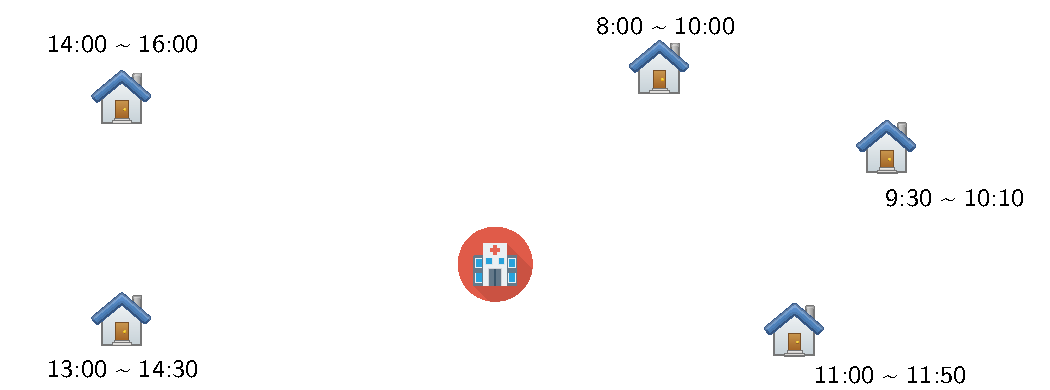
\includegraphics[width=0.8\textwidth, page=1]{fig/routing-example}%
      \end{figure}
   }

   \only<+> {
      \begin{figure}[H]
         \includegraphics[width=0.8\textwidth, page=2]{fig/routing-example}%
      \end{figure}
   }

   \only<+> {
      \begin{figure}[H]
         \includegraphics[width=0.8\textwidth, page=3]{fig/routing-example}%
      \end{figure}
   }

   \only<+> {
      \begin{figure}[H]
         \includegraphics[width=0.8\textwidth, page=4]{fig/routing-example}%
      \end{figure}
   }

   \only<+> {
      \begin{figure}[H]
         \includegraphics[width=0.8\textwidth, page=5]{fig/routing-example}%
      \end{figure}
   }

   \only<+> {
      \begin{figure}[H]
         \includegraphics[width=0.8\textwidth, page=6]{fig/routing-example}%
      \end{figure}
   }
}

%\frame{
%   \frametitle{Logistic management for healthcare systems}
%
%   \textbf{Arriving challenge:} Efficient routing solution for caregivers to patient locations.
%
%   \begin{itemize}
%      \item Reduces hospitalization costs
%      \item Decentralized care
%      \item Increases patients comfort
%      \item Reduces patient stress and the pressure of mental health
%   \end{itemize}
%}

\frame{
   \frametitle{Logistic management for healthcare systems}

   \textbf{Increased life expectancy}

   \only<1> {
   \begin{itemize}
      \item Population aging
      \item Exhaustion of public healthcare services
   \end{itemize}
   }

   \vspace*{8pt}

   \only<1,2> {
      \begin{figure}[H]

         \subfloat[Brazil in 2010]{
            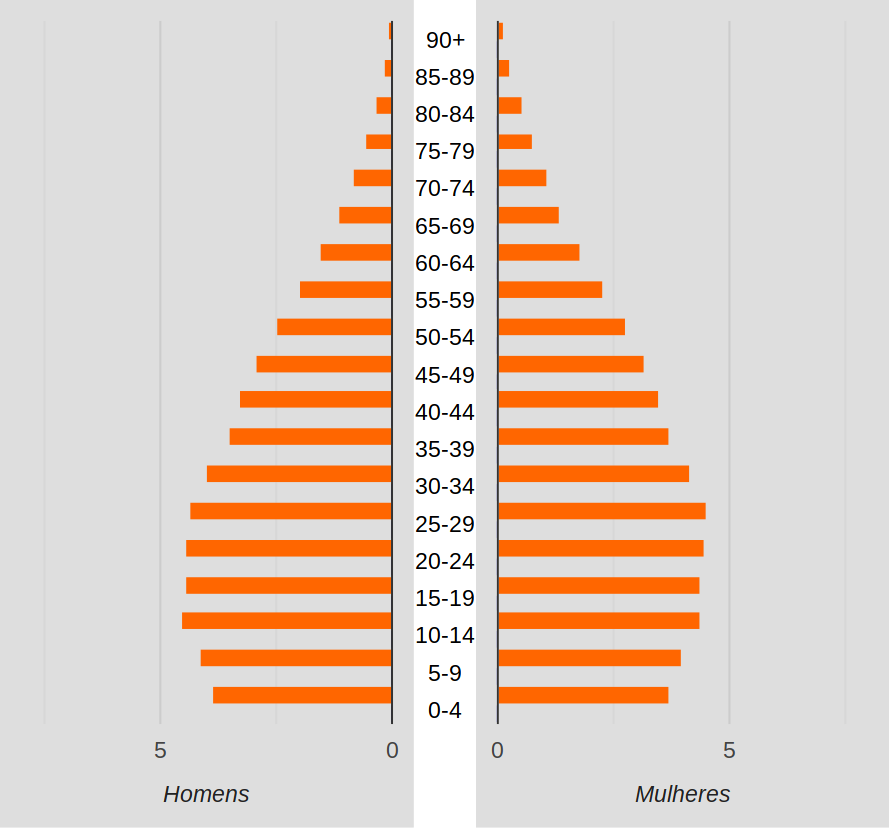
\includegraphics[width=0.29\textwidth]{fig/piramide-2010.png}

         }
         \hfill
         \subfloat[Brazil in 2021]{
           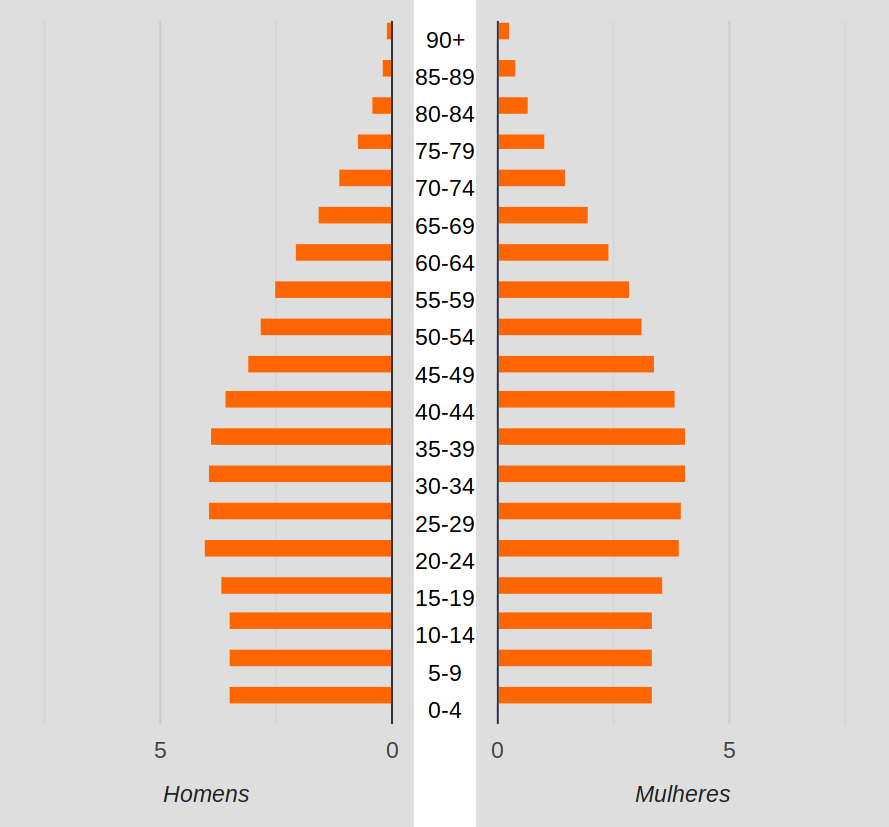
\includegraphics[width=0.29\textwidth]{fig/piramide-2021.png}

         }
         \hfill
         \subfloat[Brazil in 2050]{
            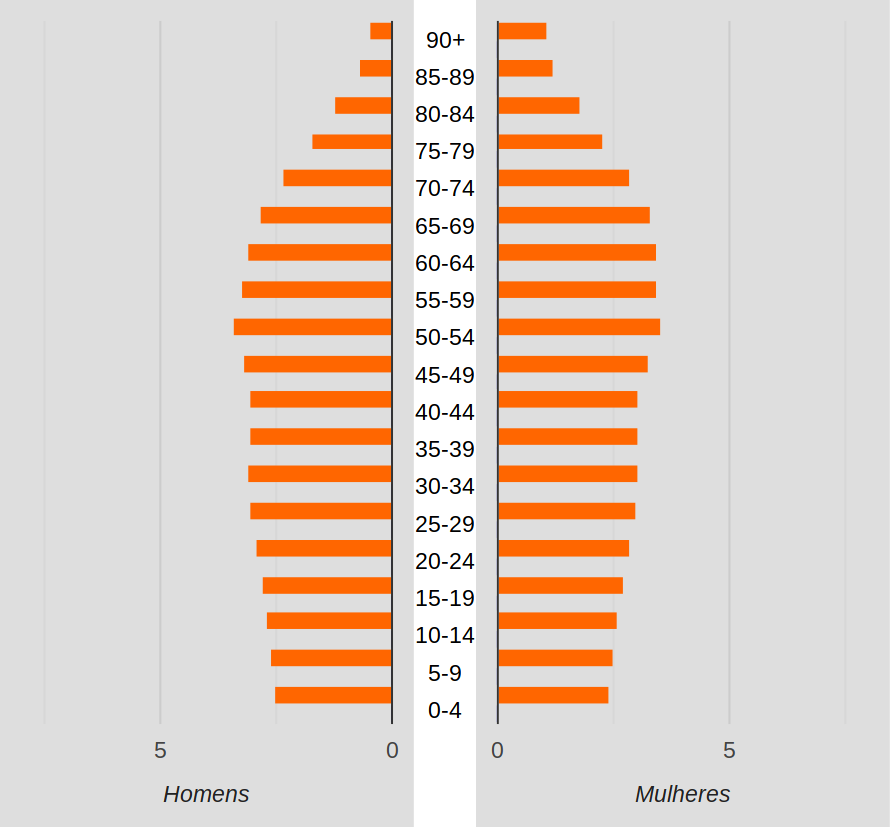
\includegraphics[width=0.29\textwidth]{fig/piramide-2050.png}

         }

         \caption{Source: Brazilian Institute of Geography and Statistics (2010)}

      \end{figure}
   }

   \only<2> {
%      \begin{figure}[H]
%         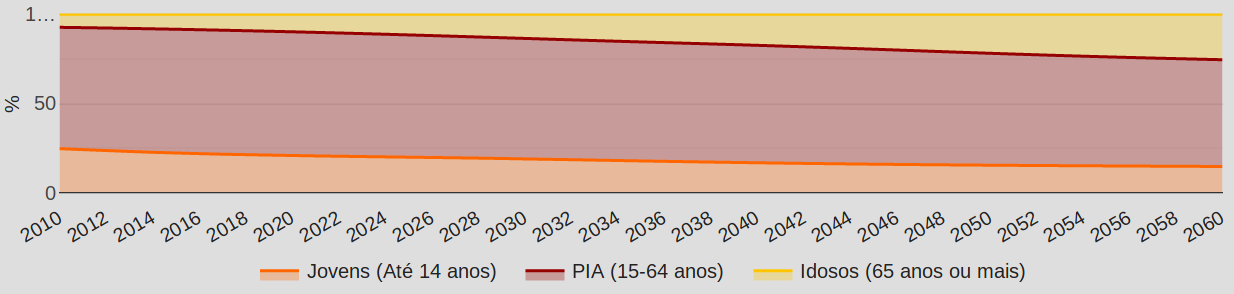
\includegraphics[width=\textwidth]{fig/brazilian-pop-evol.png}
%         \caption{Source: Brazilian Institute of Geography and Statistics (2010)}
%      \end{figure}

      Estimated population over 65+ years:
      \footnotesize
      \begin{itemize}
         \item In 2010: \phantom{0}7.32\% (14M people)
         \item In 2021: 10.15\% (21M people)
         \item In 2050: \color{InfRed} 21.87\% (51M people)
      \end{itemize}
   }
}

\frame{
   \frametitle{Logistic management for healthcare systems}

   \textbf{Healthcare services}
   \begin{itemize}
      \item Physiotherapy
      \item Dressing change
   \end{itemize}

   \vspace*{12pt}

   \textbf{Social care services}
   \begin{itemize}
      \item Preparation of meals
      \item Bathing, laundry
      \item House cleaning
   \end{itemize}
}



\frame{
   \frametitle{Logistic management for healthcare systems}

   \begin{tikzpicture}[overlay]
   \node at (9.5,-0.3) {
\includegraphics[scale=0.4]{fig/snapshot-covid}} ;
   \end{tikzpicture}

   \vspace{4pt}

   \textbf{Covid-19 pandemic in Brazil}
   \begin{figure}[H]
      \subfloat[Total cases (\textasciitilde 14M)]{
         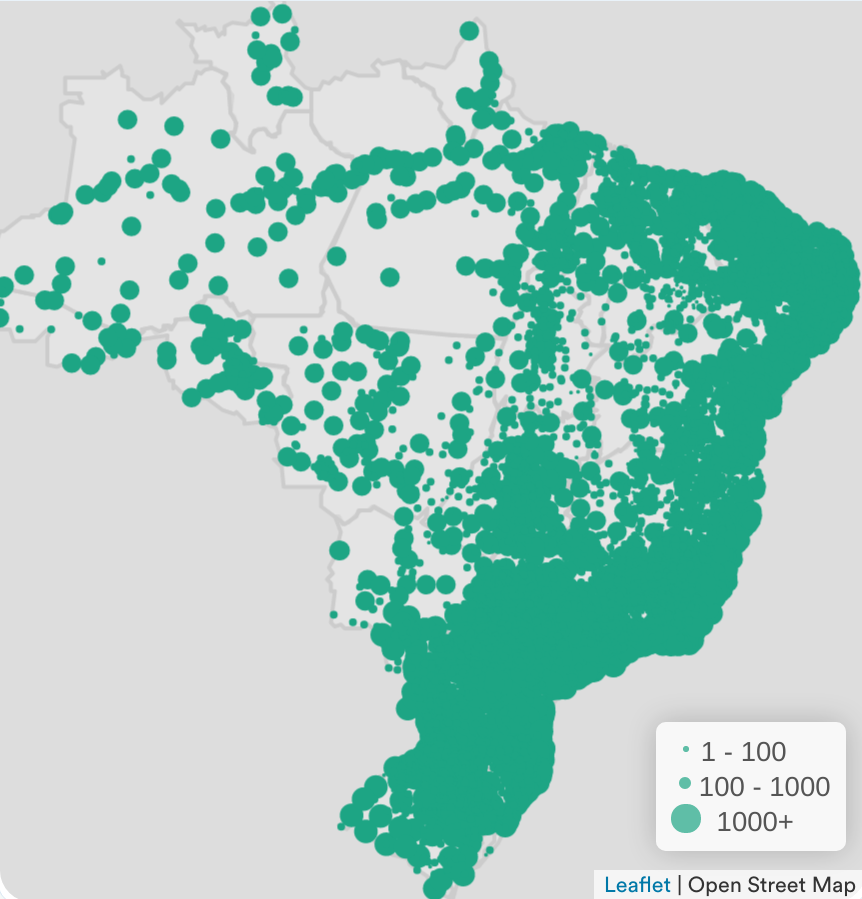
\includegraphics[width=0.4\textwidth]{fig/casos-covid}
      }
      \hfill
      \subfloat[Total deaths (\textasciitilde 378k)]{
         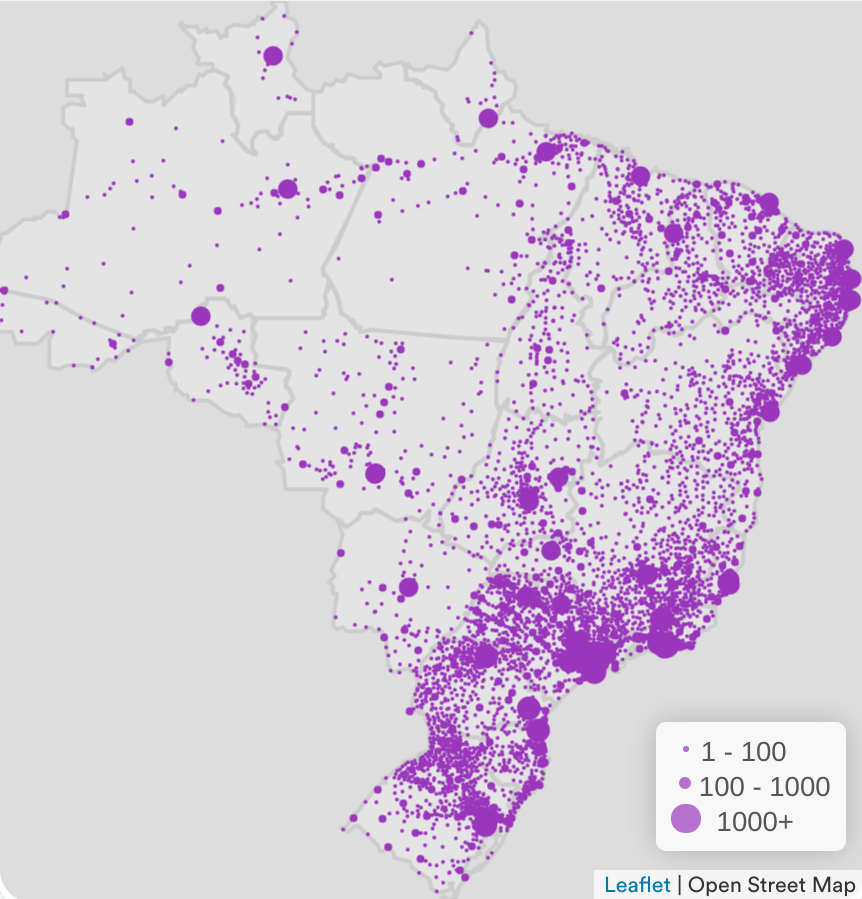
\includegraphics[width=0.4\textwidth]{fig/obitos-covid}
      }
      \caption{Source: DATASUS (2021)}
   \end{figure}
}

\frame{
   \frametitle{Logistic management for healthcare systems}

   \textbf{Covid-19 pandemic in Brazil}
   \begin{itemize}
      \item Lack of testing
      \item Lack of monitoring
   \end{itemize}

   \vspace{12pt}

   \textbf{But our public health system could be doing more}
   \begin{itemize}
      \item \emph{Better in Home}: pilot HHC program
%      \item Before the pandemic: weekly visit by health agents
      \item In Porto Alegre: vaccination through HHC structure
   \end{itemize}
}


\section{Related works}

\begin{frame}[plain]
   \sectionpage
\end{frame}


\frame{
   \frametitle{Literature outline}

   \textbf{In general}
   \begin{itemize}
      \item Most publications approach \emph{only} the routing problem \citep{gutierrez2013,grieco2020}
      \item Three surveys on routing problems arriving HHCP: \citet{fikar2017}, \citet{cisse2017}, and \citet{grieco2020}
      \item This is also the case of this thesis proposal
   \end{itemize}
}

\frame{
   \frametitle{Literature outline}

   \textbf{HHC involves much more than routing and scheduling}
   \begin{itemize}
      \item Placement of operation centers
      \item Choice of health and social services offered
      \item Staffing and supplier selection
      \item Fleet assignment and staff routing
      \item Inventory management
   \end{itemize}

    \vspace*{12pt}

   \textbf{Lots of similarities with supply chain and task workforce problems \citep{ballou2007,castillo2016}}
%   \begin{itemize}
%      \item Strategical planning
%      \item Tactical planning
%      \item Operational planning
%   \end{itemize}
}

\frame{
   \frametitle[plain]{Literature outline}

   \begin{center}
      \begin{adjustbox}{width=0.6\textwidth}

      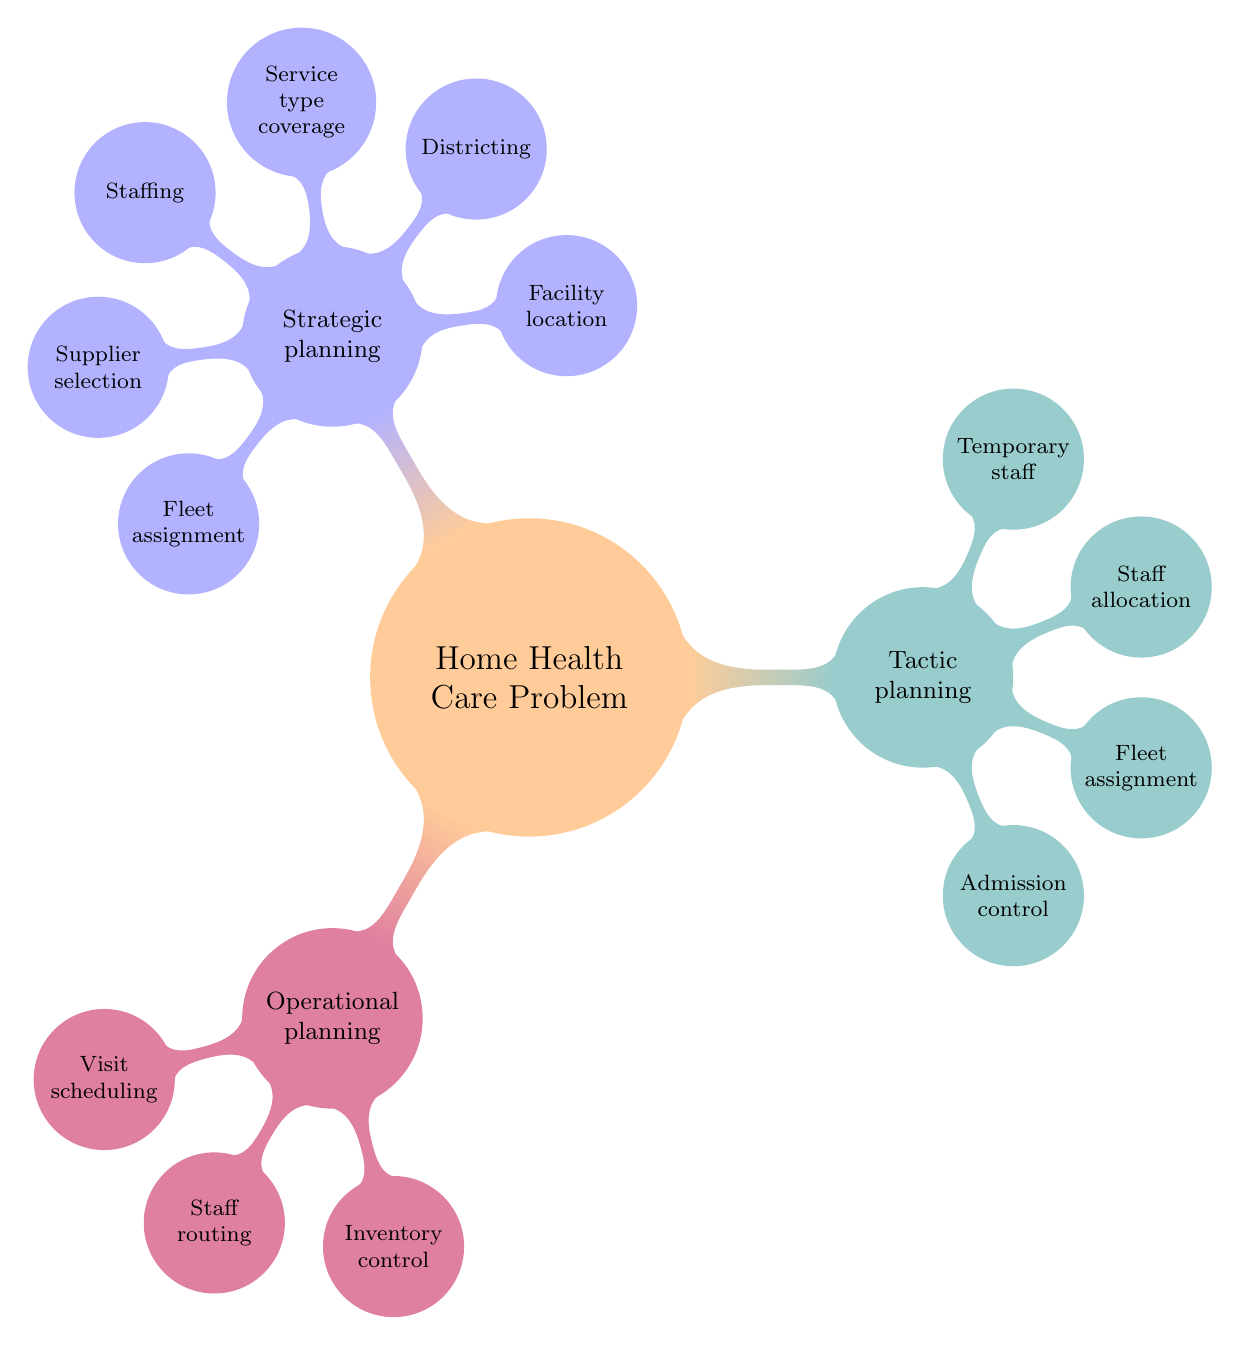
\begin{tikzpicture}[mindmap, grow cyclic, every node/.style=concept, concept color=orange!40,
      level 1/.append style={level distance=5cm,sibling angle=120},
      level 2/.append style={level distance=3cm,sibling angle=45}]

         \node{  Home Health Care Problem}
         child [concept color=purple!50] { node {  Operational planning}
            child { node {Visit scheduling}}
            child { node {Staff routing}}
            child { node {Inventory control}}
         }
         child [concept color=teal!40] { node {  Tactic planning}
            child { node {Admission control}}
            child { node {Fleet assignment}}
            child { node {Staff allocation}}
            child { node {Temporary staff}}
         }
         child [concept color=blue!30] { node { Strategic planning}
            child { node {Facility location}}
            child { node {Districting}}
            child { node {Service type coverage}}
            child { node {Staffing}}
            child { node {Supplier selection}}
            child { node {Fleet assignment}}
         };
      \end{tikzpicture}
      \end{adjustbox}
      \\[2pt]
      \footnotesize
      Source: based on the work of \citet{gutierrez2013}.
   \end{center}
}

\frame{
   \frametitle{Operational planning for the HHCP}

   \textbf{Basic definition as a routing problem}
   \begin{itemize}
%      \item \citet{fernandez1974} studied the problem through statistics
      \item Model introduced by \citet{cheng1998}
%      \item Generalization of vehicle routing problem with time-windows \citep{akjiratikarl2007}
      \item Travel times between all pairs of locations
      \item Service times, patients time-windows
   \end{itemize}

}



\frame{
   \frametitle{Operational planning for the HHCP}

   \textbf{Also a rich research subtopic}
   \footnotesize
   \begin{itemize}
      \item Planning horizon length
      \item Working regulations
      \item {Preferences}
      \item {Uncertainty}
      \item Multiple services types
      \item Multiple visits, operations synchronization
      \item \citet{fikar2017}, \citet{cisse2017}, \citet{grieco2020}
   \end{itemize}
   \normalsize

   \vspace*{12pt}

   \textbf{Integrated approaches}
   \footnotesize
   \begin{itemize}
      \item Fluctuation demands and temporary hiring \citep{eveborn2006}
      \item Fleeting and operational planning \citep{fikar2018}
   \end{itemize}
   \normalsize
}

\section{Problem definition}

\begin{frame}[plain]
   \sectionpage
\end{frame}

\begin{frame}
   \frametitle{Our target problem}

   \textbf{Seeking for a \emph{core} optimization problem}
   \begin{itemize}
%      \item No standard instance dataset \citep{fikar2017, grenouilleau2020}
      \item Complex ``enough''
      \item Not too much constrained/specific
   \end{itemize}

   \vspace*{12pt}

   \textbf{The home health care routing and scheduling problem}
   \begin{itemize}
      \item HHCRSP was introduced by \citet{mankowska2014}
      \item Routing (caregivers) and scheduling (visit time)
      \item A model, and heuristics
      \item A public standard benchmark dataset
   \end{itemize}

%   \vspace{20pt}

%   \centering\includegraphics[width=0.9\textwidth]{img/skilled}

\end{frame}

\frame{
   \frametitle{The HHCRSP}

   \textbf{Main characteristics}
   \begin{enumerate}
      \item Routing components
      \item Patient time-window
      \item Covered service types
      \item Operations synchronization on multiple visits
   \end{enumerate}
}

\frame{
   \frametitle{The HHCRSP}

   \textbf{Main characteristics}
   \begin{enumerate}
      \item \textcolor{InfRed}{Routing components}
      \item Patient time-window
      \item Covered service types
      \item Operations synchronization on multiple visits
   \end{enumerate}
}

\frame{
   \frametitle{The HHCRSP: Routing features}
   \textbf{Routing components}
   \begin{itemize}
      \item Single transportation mode
      \item Routes start and finish at the depot
      \item Travel time between locations
      \item All visits must be performed
   \end{itemize}

%   \vspace*{12pt}

   \begin{figure}
      \includegraphics[width=0.9\textwidth,page=7]{fig/routing-example}
   \end{figure}
}

\frame{
   \frametitle{The HHCRSP}

   \textbf{Main characteristics}
   \begin{enumerate}
      \item \onlyh{1}{InfRed}{Routing components}
      \item \onlyh{2}{InfRed}{Patient time-window}
      \item Covered service types
      \item Operations synchronization on multiple visits
   \end{enumerate}
}

\frame{
   \frametitle{The HHCRSP: Routing features}
   \textbf{Soft time-window}
   \begin{itemize}
      \item Each patient/node has a time-window
      \item ``Hard'' time-window start
      \item ``Soft'' time-window ending
      \item Violated time-window ending: incurs additional cost
   \end{itemize}

   \begin{figure}[H]
      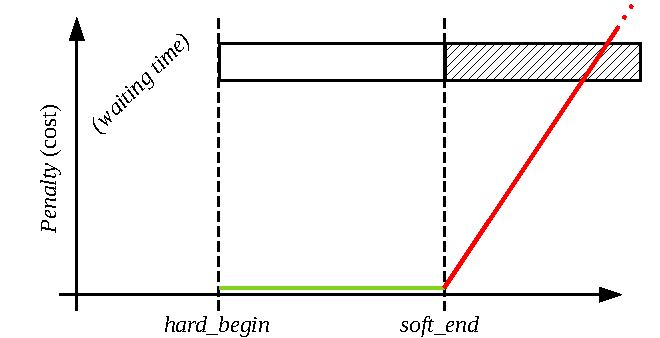
\includegraphics[width=0.7\textwidth]{fig/tw-penal.pdf}
   \end{figure}
}

\frame{
   \frametitle{The HHCRSP}

   \textbf{Main characteristics}
   \begin{enumerate}
      \item Routing components
      \item \onlyh{1}{InfRed}{Patient time-window}
      \item \onlyh{2}{InfRed}{Covered service types}
      \item Operations synchronization on multiple visits
   \end{enumerate}
}

\frame{
   \frametitle{The HHCRSP: domain features}

   \textbf{Covered service types}
   \begin{itemize}
      \item Set $\Sk$ of offered services
      \item A patient can require \textit{one}, or \textit{two services}
      \item Each service requested has a \textit{processing time}
      \item Caregivers have \textit{qualification} to perform only a few service types
   \end{itemize}

   \vspace*{8pt}

    \begin{figure}[H]
      \includegraphics[width=0.9\textwidth]{fig/skilled}
   \end{figure}

}

\frame{
   \frametitle{The HHCRSP}

   \textbf{Main characteristics}
   \begin{enumerate}
      \item Routing components
      \item Patient time-window
      \item \onlyh{1}{InfRed}{Covered service types}
      \item \onlyh{2}{InfRed}{Operations synchronization on multiple visits}
   \end{enumerate}
}


\begin{frame}
   \frametitle{The HHCRSP: domain features}
   \textbf{Operations synchronization on double service patients}
   \begin{itemize}
      \item Special requirement for patients requiring two service types
      \item Services must start simultaneously in some patients
      \item Others have precedence constraints
      \item Common feature container allocation/transshipment problems \citep{drexl2012synchronization}
   \end{itemize}

%   \vspace*{8pt}

   \begin{figure}[H]
      \includegraphics[width=1\textwidth,page=2]{fig/skilled}
   \end{figure}

\end{frame}

\begin{frame}
   \frametitle{The HHCRSP: Own characteristics}
   \textbf{Double service: precedence order}
   \begin{itemize}
      \item Service precedence: 2 > 5
      \item ($\delta^\mathrm{min}$) and ($\delta^\mathrm{max}$): separation time
   \end{itemize}

   \begin{figure}
      \centering
      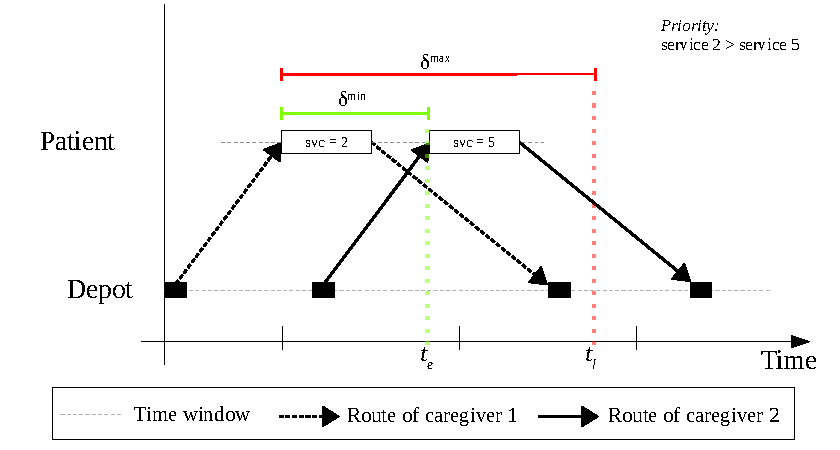
\includegraphics[width=0.8\textwidth,page=1]{fig/sync-tsn2}
   \end{figure}
\end{frame}

\begin{frame}
   \frametitle{The HHCRSP: Own characteristics}
   \textbf{Double service: parallel attendance}
   \begin{itemize}
      \item Services must start simultaneously
   \end{itemize}

   \begin{figure}
      \centering
      \includegraphics[width=0.8\textwidth,page=2]{fig/sync-tsn2}
   \end{figure}
\end{frame}

\begin{frame}
   \frametitle{The HHCRSP: some formal definitions}
   \textbf{Main sets}
   \begin{itemize}
      \item $\mathcal{V}$ : Vehicles/caregivers
      \item $\mathcal{C}$ : Patients/nodes
      \item $\mathcal{S}$ : Service types/skills
   \end{itemize}

\end{frame}

\frame{
   \frametitle{The HHCRSP: some formal definitions}

   \textbf{Objective function}

   \only<1> {
      \begin{gather}
         \mathrm{Minimize~} \lambda_1 D \; +
         \lambda_2 T \; +
         \lambda_3 T^\mathit{max} \nonumber
      \end{gather}
   }

   \only<2-5> {
      \begin{gather}
      \mathrm{Minimize~}\color{InfRed} \lambda_1 \normalcolor D \; +
      \color{green} \lambda_2 \normalcolor T \; +
      \color{blue} \lambda_3 \normalcolor T^\mathit{max} \nonumber
      \end{gather}
   }

   \vspace*{12pt}

   \textbf{Components}
   \begin{itemize}
      \item $D$: Sum of traveled distance
      \item $T$: Sum of tardiness
      \item $T^\mathrm{max}$: Maximum tardiness
   \end{itemize}

   \begin{tikzpicture}[overlay]
      \draw<3>[InfRed,line width=2pt] (4.3,3.4) rectangle +(0.9, 0.7);
      \draw<3>[InfRed,line width=2pt] (-0.4, 1.54) rectangle +(6.4, 0.7);
      \draw<4>[InfRed,line width=2pt] (5.55,3.4) rectangle +(0.9, 0.7);
      \draw<4>[InfRed,line width=2pt] (-0.4, 0.95) rectangle +(6.4, 0.7);
      \draw<5>[InfRed,line width=2pt] (6.85, 3.4) rectangle +(1.3, 0.7);
      \draw<5>[InfRed,line width=2pt] (-0.4, 0.35) rectangle +(6.4, 0.7);
   \end{tikzpicture}
}

\section{Proposed methods}

\begin{frame}[plain]
   \sectionpage
\end{frame}

\frame{
   \frametitle{Outline}

   \textbf{Model-based approaches}
   \begin{itemize}
      \item \onlyh{2}{InfRed}{Improved lower bounds}
      \item Fix-and-optimize \emph{matheuristic}
   \end{itemize}

   \vspace*{24pt}

   \textbf{Meta-heuristic approaches}
   \begin{itemize}
      \item A biased random key genetic algorithm
      \item BRKGA with additional intensification components
   \end{itemize}
}

\subsection*{Model-based approaches}


\frame{
   \frametitle{Improved lower bounds}

   \textbf{Our experiments}
   \begin{itemize}
      \item MIP and objective weights of \citet{mankowska2014}
      \item Same model, \emph{smarter} building routines
      \item CPLEX 20.10 (Dec 2020)
%      \item 2 hours of processing
%      \item Single thread
%      \item Additional parameters to reduce memory consumption
%      \item MIP warm-start with one of our proposed meta-heuristics
   \end{itemize}

   \vspace{12pt}

   \textbf{Black-box tweaks}
   \begin{itemize}
      \item Additional parameters to reduce memory consumption
      \item MIP warm-start with one of our proposed meta-heuristics
   \end{itemize}

%   \begin{table}[H]
%      \centering
%      \scriptsize
%      \begin{tabular}{ll}
%         \toprule
%         Parameter & Tweaked value\\
%         \midrule
%         disable parallel processing &  \texttt{set threads 1}\\
%         turning on the reduced memory emphasis &  \texttt{set emphasis memory y}\\
%         set all cut generation to moderate &  \texttt{set mip cuts all 1}\\
%         disable clique cut generation &  \texttt{set mip cuts clique -1}\\
%         disable the probing on the root node &  \texttt{set mip strategy probe -1}\\
%         setting the branching direction to explore up first &  \texttt{set mip strategy branch 1}\\
%         setting the mip emphasis to improve the best bound &  \texttt{set emphasis mip 3}\\
%         fixing the random seed to 1 &  \texttt{set randomseed 1}\\
%         \bottomrule
%      \end{tabular}
%   \end{table}
}

\frame{
   \frametitle{Outline}

   \textbf{Model-based approaches}
   \begin{itemize}
      \item \onlyh{1}{InfRed}{Improved lower bounds}
      \item \onlyh{2}{InfRed}{Fix-and-optimize \emph{matheuristic}}
   \end{itemize}

   \vspace*{24pt}

   \textbf{Meta-heuristic approaches}
   \begin{itemize}
      \item A biased random key genetic algorithm
      \item BRKGA with additional intensification components
   \end{itemize}
}

\frame{
   \frametitle{Fix-and-Optimize \emph{matheuristic}}

   \textbf{Solving a MIP directly is very ineffective}
   \begin{itemize}
      \item Weak lower bounds \citep{gendreau2010}
      \item Feasibility issues
      \item Convergence issues
      \item Memory consumption
   \end{itemize}

   \vspace*{12pt}

   \textbf{The Fix-and-Optimize \emph{matheuristic}}
   \begin{itemize}
      \item Originally proposed by \citet{helber2010}
%      \item Applied by \citet{dorneles2014fix}
%      \item Also applied by \citet{chen2015}
      \item ``MIP-based local search''
   \end{itemize}
}

\frame{
   \frametitle{Fix-and-Optimize \emph{matheuristic}}

   \textbf{The Fix-and-Optimize \emph{matheuristic}}
   \begin{itemize}
      \item Still requires keeping the model in memory
      \item (Usually) requires a initial solution
   \end{itemize}

   \vspace*{8pt}

   % Define block styles
   \tikzstyle{decision} = [diamond, draw, fill=yellow!20,
   text width=4.5em, text badly centered, node distance=3cm, inner sep=0pt]
   \tikzstyle{block} = [rectangle, draw, fill=InfRed!20,
   text width=5em, text centered, rounded corners, minimum height=4em]
   \tikzstyle{line} = [draw, -latex']

   \begin{figure}[H]
      \centering
      \begin{tikzpicture}[node distance = 2.5cm, auto]
         \scriptsize
         \node [block] (init) {initial solution};
         \node [block, right of=init, node distance=2.8cm] (subproblem) {generate subproblem};
         \node [block, below of=subproblem] (optimize) {solver call};
         \node [decision, right of=optimize] (stop-criteria) {stop criteria achieved};
         \node [block, right of=stop-criteria, node distance=3cm] (finish) {finish};

         \path [line] (init) -- (subproblem);
         \path [line] (subproblem) -- (optimize);
         \path [line] (optimize) -- (stop-criteria);
         \path [line] (stop-criteria) |- node [near start] {no} (subproblem);
         \path [line] (stop-criteria) -- node [near start] {yes} (finish);
      \end{tikzpicture}
   \end{figure}

%   \begin{tikzpicture}[overlay]
%      \draw<2>[green,line width=2pt](-0.1, 3.6) rectangle (2.1, 5.18);
%   \end{tikzpicture}
}


%\frame{
%   \frametitle{Fix-and-Optimize \emph{matheuristic}}
%
%  \textbf{On the subproblem generation: decomposition}
%   \begin{itemize}
%      \item Removes variable fixing constraints
%      \item ``Variable unfixing''
%      \item Can remove as many constraints as desired
%   \end{itemize}
%
%   \vspace*{18pt}
%
%   \textbf{Choice of variables to unfix}
%   \begin{itemize}
%      \item Tractable subproblem
%      \item (Potentially) allowing solution improvement
%   \end{itemize}
%}
%
%\frame{
%   \frametitle{Fix-and-Optimize \emph{matheuristic}}
%
%   \textbf{The Fix-and-Optimize \emph{matheuristic}}
%   \begin{itemize}
%      \item Still requires keeping the model in memory
%      \item (Usually) requires a initial solution
%   \end{itemize}
%
%   \vspace*{8pt}
%
%   % Define block styles
%   \tikzstyle{decision} = [diamond, draw, fill=yellow!20,
%   text width=4.5em, text badly centered, node distance=3cm, inner sep=0pt]
%   \tikzstyle{block} = [rectangle, draw, fill=InfRed!20,
%   text width=5em, text centered, rounded corners, minimum height=4em]
%   \tikzstyle{line} = [draw, -latex']
%
%   \begin{figure}[H]
%      \centering
%      \begin{tikzpicture}[node distance = 2.5cm, auto]
%      \scriptsize
%      \node [block] (init) {initial solution};
%      \node [block, right of=init, node distance=2.8cm] (subproblem) {generate subproblem};
%      \node [block, below of=subproblem] (optimize) {solver call};
%      \node [decision, right of=optimize] (stop-criteria) {stop criteria achieved};
%      \node [block, right of=stop-criteria, node distance=3cm] (finish) {finish};
%
%      \path [line] (init) -- (subproblem);
%      \path [line] (subproblem) -- (optimize);
%      \path [line] (optimize) -- (stop-criteria);
%      \path [line] (stop-criteria) |- node [near start] {no} (subproblem);
%      \path [line] (stop-criteria) -- node [near start] {yes} (finish);
%      \end{tikzpicture}
%   \end{figure}
%
%   \begin{tikzpicture}[overlay]
%   \draw<1>[green,line width=2pt](2.7, 3.6) rectangle (4.91, 5.18);
%   \draw<2>[green,line width=2pt](2.7, 1.08) rectangle (4.9, 2.76);
%   \end{tikzpicture}
%}
%
%\frame{
%   \frametitle{Fix-and-Optimize \emph{matheuristic}}
%
%    \textbf{After decomposing}
%   \begin{itemize}
%      \item Calls the MIP optimizer
%      \item Usually a timeout is set (parameter ``step time limit'', or STL)
%      \item Generate new variable fixing constraints
%   \end{itemize}
%
%   \begin{tikzpicture}[overlay]
%      \draw<2>[InfRed,line width=2pt](-0.4, 0.35) rectangle (7.6, 0.98);
%      \node<2>[rectangle, fill=InfRed, anchor=south, text=white] at (3.8, -0.21) {Same solution, or a improved one};
%   \end{tikzpicture}
%}
%
%\frame{
%   \frametitle{Fix-and-Optimize \emph{matheuristic}}
%
%   \textbf{The Fix-and-Optimize \emph{matheuristic}}
%   \begin{itemize}
%      \item Still requires keeping the model in memory
%      \item (Usually) requires a initial solution
%   \end{itemize}
%
%   \vspace*{8pt}
%
%   % Define block styles
%   \tikzstyle{decision} = [diamond, draw, fill=yellow!20,
%   text width=4.5em, text badly centered, node distance=3cm, inner sep=0pt]
%   \tikzstyle{block} = [rectangle, draw, fill=InfRed!20,
%   text width=5em, text centered, rounded corners, minimum height=4em]
%   \tikzstyle{line} = [draw, -latex']
%
%   \begin{figure}[H]
%      \centering
%      \begin{tikzpicture}[node distance = 2.5cm, auto]
%      \scriptsize
%      \node [block] (init) {initial solution};
%      \node [block, right of=init, node distance=2.8cm] (subproblem) {generate subproblem};
%      \node [block, below of=subproblem] (optimize) {solver call};
%      \node [decision, right of=optimize] (stop-criteria) {stop criteria achieved};
%      \node [block, right of=stop-criteria, node distance=3cm] (finish) {finish};
%
%      \path [line] (init) -- (subproblem);
%      \path [line] (subproblem) -- (optimize);
%      \path [line] (optimize) -- (stop-criteria);
%      \path [line] (stop-criteria) |- node [near start] {no} (subproblem);
%      \path [line] (stop-criteria) -- node [near start] {yes} (finish);
%      \end{tikzpicture}
%   \end{figure}
%
%   \begin{tikzpicture}[overlay]
%      \draw<1>[green,line width=2pt](2.7, 1.08) rectangle (4.9, 2.76);
%      \draw<2>[green,line width=2pt](5.4, 0.55) rectangle (8.13, 3.15);
%   \end{tikzpicture}
%}
%
%\frame{
%   \frametitle{Fix-and-Optimize \emph{matheuristic}}
%
%   \textbf{Stopping criteria}
%   \begin{itemize}
%      \item Most common approach: iterations without improvement
%      \item Iters w/o improv: according to the size of the problem
%   \end{itemize}
%}
%
\frame{
   \frametitle{Fix-and-Optimize \emph{matheuristic}}

   \textbf{HHCRSP-specific F\&O:}
   \begin{itemize}
      \item Initial solution from \citeauthor{mankowska2014} constructive heuristic
      \item Keeps entire MIP in memory due to op. synchronizations
      \item Decomposition: optimizes \textit{two routes} at each iteration
   \end{itemize}

   \vspace*{12pt}

%   \textbf{Routes selection: selects caregivers $v_1 \neq v_2 \in \V$}
%   \begin{itemize}
%      \item At random (originally \emph{systematic decomposition})
%      \item Or guided, according patients' visit times
%   \end{itemize}
}

\frame{
   \frametitle{Outline}

   \textbf{Model-based approaches}
   \begin{itemize}
      \item Improved lower bounds
      \item \onlyh{1}{InfRed}{Fix-and-optimize \emph{matheuristic}}
   \end{itemize}

   \vspace*{24pt}

   \textbf{Meta-heuristic approaches}
   \begin{itemize}
      \item \onlyh{2}{InfRed}{A biased random key genetic algorithm}
      \item BRKGA with additional intensification components
   \end{itemize}
}

\subsection*{Meta-heuristic approaches}

\frame{
   \frametitle{Biased random key genetic alg.}

   \textbf{Base concept of RKGAs}
   \begin{itemize}
      \item Proposed by \citet{bean1994}
      \item Indirect representation
      \item Generic GA, needs a decoder
   \end{itemize}

   \begin{figure}[H]
      \centering
      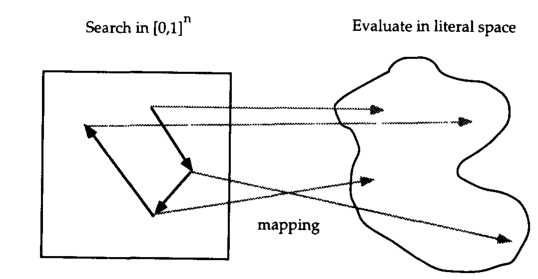
\includegraphics[width=0.6\textwidth]{fig/bean1994-rkga-decode.pdf}\\
      \footnotesize Source: \citet{bean1994}
   \end{figure}

%   \begin{tikzpicture}[overlay]
%      \draw<2,3>[green,line width=2pt](2.5, 1.26) rectangle (5.08, 4.5);
%      \node<3>[rectangle, fill=green, anchor=south, text=black] at (3.5, -0.21) {$v = \left(0.46 \quad 0.91 \quad 0.33 \quad 0.75 \quad 0.51\right)$};
%
%      \draw<5>[green,line width=2pt](6, 1.1) rectangle (8.76, 4.5);
%      \draw<4>[green,line width=2pt](5.1, 1.6) rectangle (6.1, 2.1);
%   \end{tikzpicture}
}


%\frame{
%   \frametitle{Biased random key genetic alg.}
%
%   \textbf{Elitism to improve convergence algorithm}
%   \begin{itemize}
%      \item So-called biased random key genetic algorithm \citep{gonccalves2011}
%      \item Split the population into elite and non-elite set
%      \item The elite set is kept from one generation to the next one
%%      \item As \emph{Monotonic} search
%      \item Improved crossover algorithm
%   \end{itemize}
%}
%
%\frame{
%   \frametitle{Biased random key genetic alg.}
%
%   \textbf{Basics elements of a BRKGA}
%   \begin{itemize}
%      \item \onlyh{2-4}{InfRed}{Initial population, mutants generation}
%      \item \onlyh{6-11}{InfRed}{Biased crossover, and the offspring}
%   \end{itemize}
%
%   \only<2-5>{
%      \vspace*{12pt}
%      \textbf{Initial population}
%      \begin{itemize}
%         \item \onlyh{3-4}{InfRed}{One can \emph{encode} a solution in random-keys space}
%         \item \onlyh{5}{InfRed}{Just sample a random number generator \texttt{PRNG(0,1)}}
%      \end{itemize}
%   }
%
%   \begin{tikzpicture}[overlay]
%      \node<4>[rectangle, fill=InfRed, anchor=south, text=white] at (3.5, -0.6) {Diversity loss, premature convergence!};
%   \end{tikzpicture}
%
%   \only<6-11>{
%      \begin{figure}[H]
%         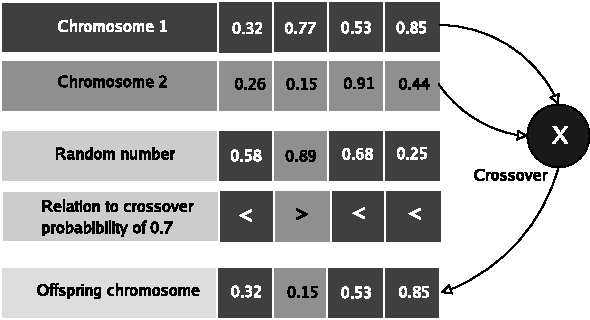
\includegraphics[width=0.7\textwidth]{fig/gonccalves2011-crossover.pdf}
%      \end{figure}
%   }
%
%   \begin{tikzpicture}[overlay]
%      \draw<7>[green,line width=2pt](1.55, 4.15) rectangle (7.35, 4.94);
%      \draw<8>[green,line width=2pt](1.55, 3.4) rectangle (7.35, 4.18);
%      \draw<9>[green,line width=2pt](4.4, 0.8) rectangle (5.13, 4.9);
%      \draw<10>[green,line width=2pt](5.13, 0.8) rectangle (5.85, 4.9);
%      \draw<11>[green,line width=2pt](1.55, 0.8) rectangle (7.35, 1.503);
%
%      \node<6-> at (5,0.3) {\footnotesize Source: \citet{gonccalves2011}};
%   \end{tikzpicture}
%}



\frame{
   \frametitle{Biased random key genetic alg.}

   \textbf{BRKGA}
   \begin{itemize}
      \item Proposed by \citet{gonccalves2011}
   \end{itemize}

   \vspace*{8pt}

   \begin{figure}[H]
      \centering
      \includegraphics[width=0.7\textwidth, page=2]{fig/brkga-framewk.pdf}
   \end{figure}
}

\frame{
   \frametitle{Biased random key genetic alg.}

   \textbf{For the home health care problem}
   \begin{itemize}
      \item BRKGA $\Rightarrow$ evolves the \emph{task insertion sequence}
      \item The proposed decoder \textbf{embeds} a greedy heuristic
      \item A \emph{best-insertion heuristic decoder} builds a routing solution from the TIS
   \end{itemize}

   \vspace*{12pt}

   \begin{figure}
      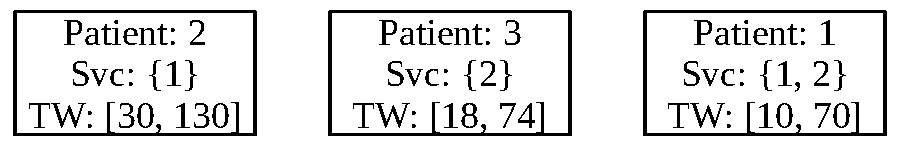
\includegraphics[width=0.6\textwidth]{fig/decoder-tis}
   \end{figure}

}

%\frame{
%   \frametitle{Biased random key genetic alg.}
%
%   \textbf{The task insertion sequence}
%   \begin{itemize}
%      \item Chromosome has many alleles than $|\C|$
%      \item Each allele represents a patient (and all their service requests)
%   \end{itemize}
%
%   \only<+> {
%      \vspace*{12pt}
%
%      \begin{figure}[H]
%         \centering
%         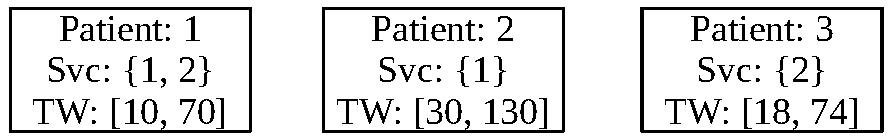
\includegraphics[width=0.7\textwidth]{fig/decoder-tasks.pdf}
%      \end{figure}
%
%      \begin{align*}
%         v = \left( 0.48 \quad 0.16 \quad 0.31 \right)
%      \end{align*}
%   }
%
%   \only<+> {
%      \vspace*{12pt}
%      \begin{figure}[H]
%         \centering
%         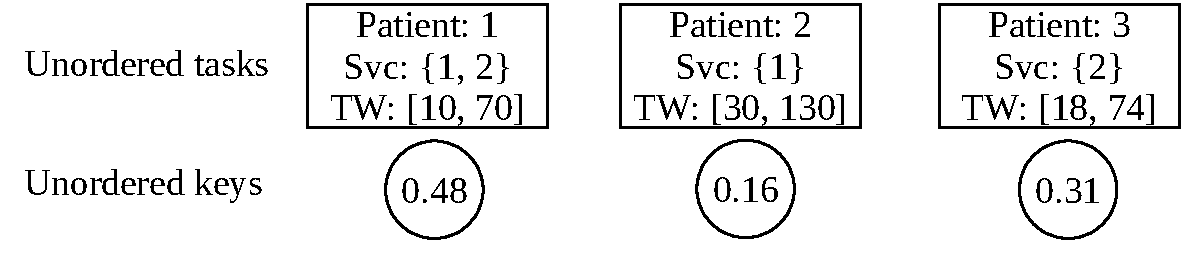
\includegraphics[width=0.8\textwidth]{fig/decoder-keys}
%      \end{figure}
%   }
%
%   \only<+> {
%      \vspace*{12pt}
%      \begin{figure}[H]
%         \centering
%         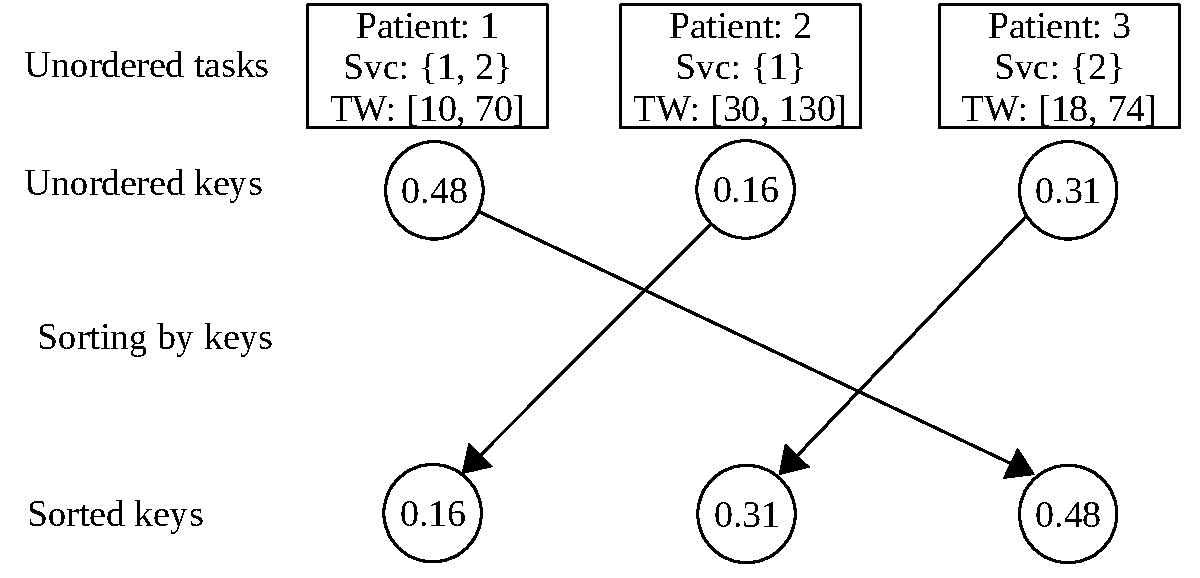
\includegraphics[width=0.8\textwidth]{fig/decoder-sort}
%      \end{figure}
%
%      \begin{tikzpicture}[overlay]
%         \draw[green,line width=2pt](1.2, 2.2) rectangle (3.2, 2.8);
%      \end{tikzpicture}
%   }
%
%   \only<+> {
%      \vspace*{12pt}
%      \begin{figure}[H]
%         \centering
%         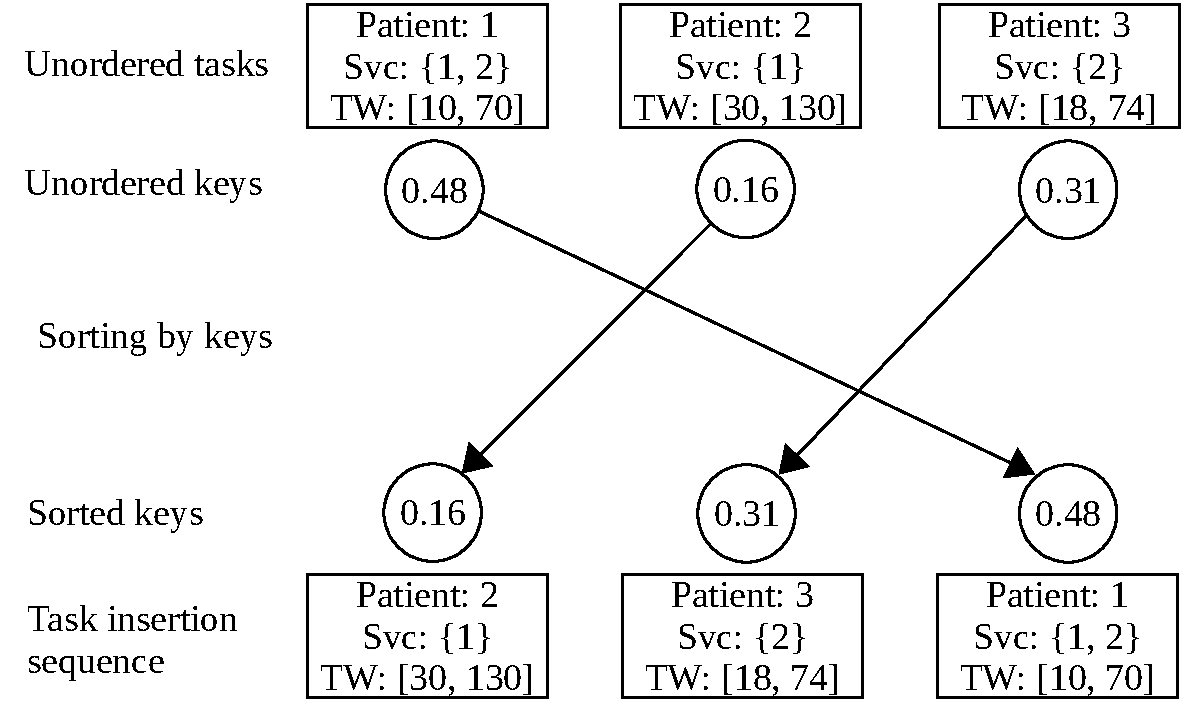
\includegraphics[width=0.8\textwidth]{fig/decoder}
%      \end{figure}
%   }
%
%%   \only<+>{
%%      \vspace*{12pt}
%%      \begin{figure}[H]
%%         \centering
%%         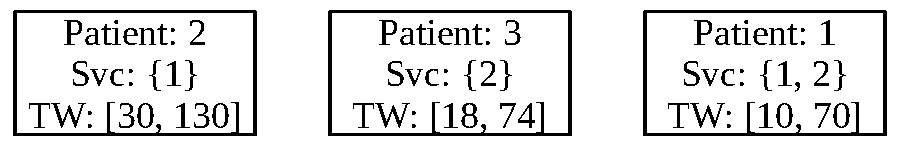
\includegraphics[width=0.8\textwidth]{fig/decoder-tis}
%%      \end{figure}
%%   }
%
%}

%\frame{
%   \frametitle{Biased random key genetic alg.}
%
%   \textbf{Best-insertion heuristic}
%   \begin{itemize}
%      \item Input: the task insertion sequence
%      \item All caregivers start at the depot
%      \item Greedily insert patient on caregiver routes
%      \item Finishes all routes at the depot
%   \end{itemize}
%
%   \vspace*{12pt}
%%
%%   \textbf{Guide the insertion according the objective function}
%%   \begin{itemize}
%%      \item Increment of travel times
%%      \item Increment of total tardiness
%%      \item Change of the maximum tardiness
%%      \item Terms combined according the weights $\lambda_1$, $\lambda_2$, and $\lambda_3$
%%   \end{itemize}
%
%
%
%}

%\frame{
%   \frametitle{Biased random key genetic alg.}
%
%   \textbf{Task insertion sequence}
%   \begin{figure}[H]
%      \centering
%      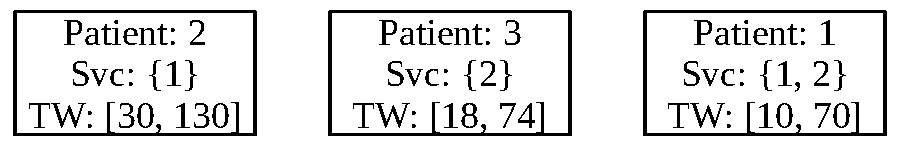
\includegraphics[width=0.6\textwidth]{fig/decoder-tis}
%   \end{figure}
%
%   \vspace*{8pt}
%
%
%   \textbf{Best-insertion heuristic}
%   \begin{figure}
%      \includegraphics<+>[width=0.95\textwidth,page=1]{fig/bi-heur}%
%      \includegraphics<+>[width=0.95\textwidth,page=2]{fig/bi-heur}%
%      \includegraphics<+>[width=0.95\textwidth,page=3]{fig/bi-heur}%
%      \includegraphics<+>[width=0.95\textwidth,page=4]{fig/bi-heur}%
%      \includegraphics<+>[width=0.95\textwidth,page=5]{fig/bi-heur}%
%      \includegraphics<+>[width=0.95\textwidth,page=6]{fig/bi-heur}%
%      \includegraphics<+>[width=0.95\textwidth,page=7]{fig/bi-heur}%
%      \includegraphics<+>[width=0.95\textwidth,page=8]{fig/bi-heur}%
%      \includegraphics<+>[width=0.95\textwidth,page=9]{fig/bi-heur}%
%      \includegraphics<+>[width=0.95\textwidth,page=10]{fig/bi-heur}%
%   \end{figure}
%
%%   \Todo{Incluir highlight no TIS durante a animação.}
%%   \Todo{Verificar se vale a pena inserir um terceiro \textit{caregiver} para demonstrar o comportamento do algoritmo.}
%}
%
%\frame{
%   \frametitle{Biased random key genetic alg.}
%
%   \textbf{Best-insertion heuristic}
%   \begin{itemize}
%      \item Consider caregiver qualification levels
%      \item Deals with double service patients
%%      \item Compute the shortest waiting times
%   \end{itemize}
%
%
%}

%\frame{
%   \frametitle{Biased random key genetic alg.}
%
%   \textbf{Best-insertion heuristic}
%   \begin{itemize}
%      \item It is not very expensive for small instances
%      \item $n = |\C|$, $m = |\V|$
%      \item Worst-case complexity of $O(nm^2)$
%      \item In practice, the cost is not so bad
%   \end{itemize}
%
%   \vspace*{8pt}
%
%   \begin{table}[H]
%      \footnotesize
%      \begin{tabular}{rrrr}
%         \toprule
%         $|\C|$ & $|\V|$ & Worst case & Empirical measure\\
%         \midrule
%         10 & 3 & 90 & 14\\
%         50 & 10 & 5,000 & 414 \\
%         100 & 20 & 40,000 & 2,571\\
%         200 & 30 & 180,000 & 12,892\\
%         300 & 40 & 480,000 & 26,996 \\ % 5.62\%  0.29 seconds 1 generation
%         \bottomrule
%      \end{tabular}
%   \end{table}
%}
%
%\frame{
%   \frametitle{Biased random key genetic alg.}
%
%   \textbf{Not always a bed of roses}
%   \begin{itemize}
%      \item The best-insertion heuristic is \textit{incomplete}
%      \item In some cases, it can not reach the optimal solution
%      \item Even though we known the optimal TIS
%   \end{itemize}
%
%   \vspace*{12pt}
%   \begin{figure}
%      \includegraphics<+>[width=0.4\textwidth, page=1]{fig/triangle.pdf}%
%      \includegraphics<+>[width=0.4\textwidth, page=2]{fig/triangle.pdf}%
%      \includegraphics<+>[width=0.4\textwidth, page=3]{fig/triangle.pdf}%
%      \only<+>{
%         \includegraphics[width=0.4\textwidth, page=4]{fig/triangle.pdf}\\
%         \footnotesize The final solution... \normalsize
%      }
%      \only<+>{
%         \includegraphics[width=0.4\textwidth, page=5]{fig/triangle.pdf}\\
%         \footnotesize ...but not the optimal one! \normalsize
%      }
%   \end{figure}
%}



\frame{
   \frametitle{Outline}

   \textbf{Model-based approaches}
   \begin{itemize}
      \item Improved lower bounds
      \item Fix-and-optimize \emph{matheuristic}
   \end{itemize}

   \vspace*{24pt}

   \textbf{Meta-heuristic approaches}
   \only<+> {
      \begin{itemize}
         \item \textcolor{InfRed}{A biased random key genetic algorithm}
         \item BRKGA with additional intensification components
      \end{itemize}
   }%
  \only<+> {
      \begin{itemize}
         \item A biased random key genetic algorithm
         \item \textcolor{InfRed}{BRKGA with additional intensification components}
      \end{itemize}
   }%
}

\frame{
   \frametitle{\footnotesize BRKGA with Intensification components}

   \textbf{Components of \citet{andrade2021}}
   \begin{enumerate}
      \item \onlyh{2}{InfRed}{Island model (also in \citet{toso2015})}
      \item Multi-parent mating
      \item Implicit path-relinking heuristic
   \end{enumerate}
}

\frame{
   \frametitle{\footnotesize BRKGA with Intensification components}

   \textbf{Island model}
   \begin{itemize}
      \item Island = a isolated population evolving by itself
      \item Standard BRKGA: single island
   \end{itemize}

   \vspace*{12pt}

   \textbf{Advantages}

   \begin{itemize}
      \item Immigration $\rightarrow$ Can find better solutions
      \item Helps keeping the diversity
      \item Shows better convergence than single-island approach
   \end{itemize}

   \vspace*{12pt}

   \textbf{Caveat: substantially more individuals to decode.}
}

\frame{
   \frametitle{\footnotesize BRKGA with Intensification components}

   \textbf{Components of \citet{andrade2021}}
   \begin{enumerate}
      \item \onlyh{1}{InfRed}{Island model (also in \citet{toso2015})}
      \item \onlyh{2}{InfRed}{Multi-parent mating}
      \item Implicit path-relinking heuristic
   \end{enumerate}
}

\frame{
   \frametitle{\footnotesize BRKGA with Intensification components}

   \textbf{Multi-parent mating}
%   \footnotesize
   \begin{itemize}
      \item Originally proposed by \citet{lucena2014-gd-mp}
      \item Objective: exploit good solution parts from several parents
      \item At least one elite parent
      \item At least one non-elite parent
      \item Implicit bias through weight functions of \citet{bresina1996-bias}
   \end{itemize}
%   \normalsize

%   \vspace*{12pt}
%   \textbf{Algorithmic view}
%   \footnotesize
%   \begin{enumerate}
%      \item Parent selection
%      \item Sort selected parents
%      \item Compute parent weight according to their \textit{rank}
%      \item Normalize the weights
%      \item Proceeds with a slightly modified mating algorithm of \citet{bean1994}
%   \end{enumerate}
%   \normalsize
}

%\frame{
%
%   \Todo{Acho que vale a pena adicionar um slide mostrando esse weight function operando no crossover}
%
%}

%\frame{
%   \frametitle{\footnotesize BRKGA with Intensification components}
%
%   \textbf{Path-relinking heuristic}
%%   \footnotesize
%   \begin{itemize}
%      \item Introduced by \citet{glover1997-pr}
%      \item Further discussed by \citet{resende2016-pr}
%      \item Acts as a \emph{directed} local-search algorithm
%   \end{itemize}
%%   \normalsize
%
%   \vspace*{12pt}
%
%   \textbf{Explore intermediate solutions}
%%   \footnotesize
%   \begin{itemize}
%      \item Common terminology: guide solution $g$, initial (or base) solution $b$
%      \item Incrementally replaces elements of $b$ with elements from $g$
%      \item Records the best solution found
%   \end{itemize}
%%   \normalsize
%
%}

\frame{
   \frametitle{\footnotesize BRKGA with Intensification components}

   \textbf{Components of \citet{andrade2021}}
   \begin{enumerate}
      \item Island model (also in \citet{toso2015})
      \item \onlyh{1}{InfRed}{Multi-parent mating}
      \item \onlyh{2}{InfRed}{Implicit path-relinking heuristic}
   \end{enumerate}
}

\frame{
   \frametitle{\footnotesize BRKGA with Intensification components}

   \textbf{Difficulties of implementing a PR}
   \begin{itemize}
      \item Efficient implementation can be challenging
      \item Variations of PR
      \item Hard to reuse: problem-dependent neighborhood
   \end{itemize}

   \vspace*{12pt}

   \textbf{Implicit path relinking come to the rescue!}
   \begin{itemize}
      \item Explores the solution space \textit{indirectly}
      \item Solutions encoded in random keys
   \end{itemize}
}

%\frame{
%   \frametitle{\footnotesize BRKGA with Intensification components}
%
%   \textbf{BRKGA with IPR}
%   \begin{itemize}
%%      \item Proposed by \citet{andrade2021}
%      \item Specialized IPR according to solution representation
%      \item In the case of the HHCRSP: permutation IPR
%   \end{itemize}
%
%   \vspace*{12pt}
%   \textbf{Permutation IPR}
%   \begin{itemize}
%      \item Given a guide individual, and a initial (or base) individual
%      \item Introduce the permutations of one individual into the other
%      \item Operates on the level of random keys
%   \end{itemize}
%
%}

%\frame{
%   \frametitle{\footnotesize BRKGA with Intensification components}
%
%   \textbf{Permutation IPR}
%
%   \begin{figure}
%      \centering
%      \includegraphics<1-3>[width=0.6\textwidth]{fig/ipr}
%      \includegraphics<4-6>[width=0.6\textwidth, page=2]{fig/ipr}
%   \end{figure}
%
%   \begin{tikzpicture}[overlay]
%%      \draw<+>[green,line width=2pt](2.8, 4.9) rectangle (8.8, 6);
%      \draw<2,3>[green,line width=2pt](3.605, 0.95) rectangle (4.65, 3.1
%      );
%      \draw<5,6>[green,line width=2pt](3.67, 0.95) rectangle (4.65, 3.1
%      );
%      \node<3>[rectangle, fill=green, anchor=south, text=black] at (0.8, 3.2) {$\operatorname{swap}(b_1, b_5)$};
%      \node<5,6>[rectangle, fill=green, anchor=south, text=black] at (4.15, 3.1) {\checkmark};
%      \draw<6>[green,line width=2pt](2.8, 4.9) rectangle (8.8, 6
%      );
%      \node<3>[rectangle, fill=green, anchor=south, text=black] at (0.8, 3.2) {$\operatorname{swap}(b_1, b_5)$};
%      \node<6>[rectangle, fill=green, anchor=south, text=black] at (3.5, -0.5) {Continues the decoding with the modified $b'$.};
%   \end{tikzpicture}
%}
%
%\frame{
%   \frametitle{\footnotesize BRKGA with Intensification components}
%
%   \textbf{BRKGA with IPR}
%   \begin{itemize}
%      \item The process repeats for each position of the chromosome
%      \item Each intermediate solution is evaluated by the decoder
%      \item In the worst case, calls the best-insertion heuristic $|\C|$ times
%      \item Worst case cost of $O(nm^2) \cdot n = O(n^2m^2)$
%      \item But the average cost, in practice, is cheaper
%   \end{itemize}
%
%   \begin{tikzpicture}[overlay]
%      \draw<2>[green,line width=2pt](-0.4, 1) rectangle (8, 1.6
%      );
%      \node<2>[rectangle, fill=green, anchor=south, text=black] at (3.5, -1.) {Recall $n = |\C|$ and $m = |\V|$.};
%%      \draw[] (0,0) grid (10,10);
%   \end{tikzpicture}
%
%}
%
%\frame{
%   \frametitle{\footnotesize BRKGA with Intensification components}
%
%   \textbf{BRKGA with IPR}
%   \begin{itemize}
%      \item Distance metrics
%      \item Typically tries a fixed number of pairs for IPR
%%      \item Best or random selection from the elite set
%      \item On multiple islands: tries IPR between elite individuals from distinct islands
%   \end{itemize}
%}

\frame{
   \frametitle{\footnotesize BRKGA with Intensification components}

%   \begin{algorithm}[H]
%      \caption{Outline of BRKGA-MP-IPR}
%      \tiny
%      $l \gets 0$\;
%      $\mathit{bestFitness} \gets \infty$\;
%      \For{$g \gets 1$ \textbf{to} $E^\mathit{tot}$} {
%         \tcp{BRKGA operations with multi-parent mating}
%         \For{$k' \gets 1$ \textbf{to} $k$} {
%            copy the elite set to the next population of $k'$\;
%            generate new mutants\;
%            fill the next population of $k'$ with offspring\;
%         }
%
%         \If{$g \mod E^\mathit{IPR}$}{
%            run the implicit path-relinking\;
%         }
%
%         \If{$g \mod E^\mathit{XE}$}{
%            run the immigration process\;
%         }
%
%         \eIf{a improved individual was found}{
%            update $\mathit{bestFitness}$\;
%            $l \gets 0$\;
%         }{
%            $l \gets l + 1$\;
%         }
%
%         \If{$l > E^\mathit{RST}$} {
%            replace all indviduals of the new population by mutants\;
%         }
%      }
%      \KwResult{Most fitted individual found.}
%   \end{algorithm}

   \textbf{BRKGA with Multi-Parent mating and IPR}
   \begin{enumerate}
      \item Initialize all islands with random individuals
      \item Mating and mutation
      \item Run implicit PR
      \item Exchange best individuals
   \end{enumerate}
}



\section{Preliminary results}

\begin{frame}[plain]
   \sectionpage
\end{frame}


\frame{
   \frametitle{Instance dataset}

   \textbf{\citet{mankowska2014} dataset}
   \begin{itemize}
      \item Total of 70 instances available
      \item Seven instance subsets, from A to G
      \item Euclidean distances
      \item Time-windows of 2 hours % within a 10 hour planning horizon
   \end{itemize}

   \vspace*{12pt}

   \textbf{Service types}
   \begin{itemize}
      \item Fixed $\Sk = \{1, 2, 3, 4, 5, 6\}$
      \item A caregiver can perform up to 3 service types
      \item 70\% of single service patients
      \item 30\% of double services
   \end{itemize}
}

\frame{
   \frametitle{Instance dataset}

   \textbf{\citet{mankowska2014} dataset}

   \begin{table}[H]
      \centering
      \footnotesize
      \begin{tabular}{lrrrrr}
         \toprule
         Instance subset & $|\mathcal{V}|$ & $|\mathcal{C}|$ &
         Avg. cols$^*$ \\
         \toprule
         A &  3 &  10 &      2,445 \\
         B &  5 &  25 &     21,219 \\
         C & 10 &  50 &    159,429 \\
         D & 15 &  75 &    527,139 \\
         E & 20 & 100 &  1,236,846 \\
         F & 30 & 200 &  7,309,566 \\
         G & 40 & 300 & 21,818,286 \\
         \midrule
         \multicolumn{4}{c}{Total of instances: 70}\\
         \bottomrule
      \end{tabular}
   \end{table}

   \vspace*{12pt}

   Ten instances for each subset.

%   $^*$With preprocessing to skip generation of variables trivially set to 0.
}

%\frame{
%   \frametitle{Benchmark machine}
%
%   \textbf{With the F\&O \textit{matheuristic}, and BRKGA}
%   \begin{itemize}
%      \item CPLEX 12.9
%      \item Intel Core i7 3612QM at 3.1 GHz
%      \item 8 GB of memory
%      \item Single thread processing
%   \end{itemize}
%
%   \vspace*{12pt}
%
%   \textbf{With the BRKGA-MP-IPR, and LB$^+$ experiment}
%   \begin{itemize}
%      \item CPLEX 20.10
%      \item Intel Core i7 930 at 2.8 GHz
%      \item 12 GB of memory
%      \item Single thread processing (CPLEX)
%      \item Parallel decoding with 4 threads (BRKGA)
%   \end{itemize}
%}

%\frame{
%   \frametitle{Previous results from the literature}
%
%   \textbf{MIP and MH \citep{mankowska2014}}
%   \begin{itemize}
%      \item CPLEX (mostly) for providing lower bounds
%      \item Initial solutions: nearest neighbor heuristic
%      \item Solution structure: three-indexed matrix
%      \item LS operators: (inter, intra)-route $\times$ (swap, shift)
%      \item Specialized operators for single and double services
%      \item Simple LS, and the Adaptive VNS
%      \item \textit{Best improvement} with a MN heuristic
%      \item \textit{Best improvement} in adaptive phase of VNS
%   \end{itemize}
%}
%
%\frame{
%   \frametitle{Previous results from the literature}
%
%   \textbf{Meta-heuristics \citet{lasfargeas2019}}
%   \begin{itemize}
%      \item Originally proposed for the short-term HHCP
%      \item Several variations of the constructive heuristic
%      \item Repeated construction with randomization
%      \item Operators: equivalent to shif and swap operators from \citet{mankowska2014}, but only single service operators
%      \item Randomizes the choice of patients to shift/swap
%      \item But the operator order is also fixed
%      \item \textit{First improvement} is used within the VNS algorithm
%      \item Results for instances with up to 75 patients
%   \end{itemize}
%}

\frame{
   \frametitle{\footnotesize Previous results from the literature}

   \textbf{MIP and MH \citep{mankowska2014}}
   \begin{itemize}
      \item CPLEX (mostly) for providing lower bounds
      \item Several LS-based heuristics, and a VNS-based algorithm
      \item Specialized operators for single and double services
%      \item Nearest neighbor-like constructive heuristic
   \end{itemize}
}

\frame{
   \frametitle{\footnotesize Previous results from the literature}

   \textbf{Meta-heuristics of \citet{lasfargeas2019}}
   \begin{itemize}
%      \item Repeated construction with randomization
      \item VNS-based metaheuristic
      \item Similar operators than \citet{mankowska2014}
      \item Randomizes the choice of patients to shift/swap
%      \item \textit{First improvement} acceptance
%      \item Results for instances with up to 75 patients
   \end{itemize}
}

%\frame{
%   \frametitle{Environmental setup}
%
%   \textbf{Speed factor between machines}
%   \begin{itemize}
%      \item Too many experiments to replicate
%      \item Many implementation details left off
%      \item Alternative approach: use published results
%      \item But we first need to estimate the speed factor among the distinct benchmark machines
%   \end{itemize}
%
%   \vspace*{12pt}
%
%   \begin{table}[H]
%      \centering
%      \scriptsize
%      \setlength{\tabcolsep}{2.5pt}
%      \renewcommand{\arraystretch}{1.1}
%      \begin{tabular}{llrr}
%         \toprule
%         Publication & Machine description & PassMark score & Factor\\
%         \midrule
%         \citet{mankowska2014} & Intel Core at 3.40 GHz & 1884 & 1.4270\\
%         \citet{lasfargeas2019} & Intel i7 at 4.00 GHz & 2528 & 1.9750\\
%         F\&O & Intel i7-3612QM at 3.10 GHz & 1484 & 1.1559\\
%         BRKGA & Intel i7-3612QM at 3.10 GHz & 1484 & 1.1559\\
%         BRKGA-MP-IPR & Intel i7-930 at 2.80 GHz & 1280 & 1.0000\\
%         \bottomrule
%      \end{tabular}
%   \end{table}
%}

\frame{
   \frametitle{Outline}

   \begin{enumerate}
      \item \onlyh{2}{InfRed}{New lower bounds with CPLEX 20.10}
      \item New upper bounds from BRKGA and BRKGA-MP-IPR
      \item Comparison with the literature
      \item New upper bounds with the MIP
   \end{enumerate}
}

\frame{
   \frametitle{New lower bounds with CPLEX 20.10}

   \bgroup
   \begin{table}[!htb]
      \scriptsize
      \setlength{\tabcolsep}{2.5pt}
      \renewcommand{\arraystretch}{1.1}
      \centering
      \begin{tabular}{lrrrrrr}
         \toprule
         \multirow{2}[2]{*}{Instance} &
         \multicolumn{2}{c}{Previous values} &
         \multicolumn{4}{c}{New values} \\

         \cmidrule(l){2-3}
         \cmidrule(l){4-7}

         & LB$^+$ & Time (sec.)
         & LB$^+$ & Time (sec.) & Improv. (\%)
         & \# Nodes \\
         \midrule

         A & \textbf{225.2} & 5.2 & \textbf{225.2} & 1.0 & 0.0 & 846 \\
         B & 343.1 & 36,000.0 & \textbf{386.0} & 4408.2 & 13.3 & 1,129,013 \\
         C & 342.6 & 36,000.0 & \textbf{403.5} & 7200.0 & 17.7 & 48,480  \\
         D & 377.4 & 36,000.0 & \textbf{411.7} & 7200.0 & 9.0 & 5,808  \\
         E & 404.5 & 36,000.0 & \textbf{418.1} & 7200.0 & 3.4 & 654   \\
         \midrule
         F & 435.3 & 36,000.0 & \textbf{528.6} & 7200.2 & 21.9 & 507   \\
         G & 462.1 & 36,000.0 & \textbf{604.3} & 7200.6 & 30.8 & 302  \\
         \midrule
         & 370.0 & 30857.9 & 425.4 & 5772.9 & 13.7 & 169372.8\\
         \bottomrule
      \end{tabular}
   \end{table}
   \egroup

   \vspace*{12pt}

   Initial solutions from BRKGA \citep{kummer2020}.
}

\frame{
   \frametitle{Outline}

   \begin{enumerate}
      \item \onlyh{1}{InfRed}{New lower bounds with CPLEX 20.10}
      \item \onlyh{2,3}{InfRed}{New upper bounds from BRKGA and BRKGA-MP-IPR}
      \only<2->{
      \begin{enumerate}
         \item \onlyh{3}{InfRed}{Automatic algorithm configuration}
         \item Computational results
      \end{enumerate}
      }
      \item Comparison with the literature
      \item New upper bounds with the MIP
   \end{enumerate}
}


\frame{
   \frametitle{Calibrating the BRKGA}

   \textbf{Highly parameterized heuristics}
   \begin{itemize}
      \item BRKGA has five parameters
      \item Island models: +3
      \item New parameters for MP: +3
      \item IPR: +5
      \item Stagnated generations before reset +1

      \item \textbf{Total: 17 parameters}
   \end{itemize}
}

\frame{
   \frametitle{Calibrating the BRKGA}

   \textbf{Automatic algorithm configuration with \emph{irace}}
   \begin{itemize}
      \item R package, easy to use \emph{front-end}
      \item Stopping criteria $\Rightarrow$ \emph{budget}, or time limit
      \item A parameter space specification
%      \item Rules for forbidden configurations
      \item A set of train instances
   \end{itemize}

   \vspace*{12pt}

   \textbf{Advantages over manual configuration}
   \begin{itemize}
      \item Prevent human errors and bias
      \item Robust experiment
   \end{itemize}

   \color{InfRed} Starting point for newcomers: \citet{lopez2016} for irace guidance, \citet{eggensperger2019-aac-best-practices} for general advice
}

%\frame{
%   \frametitle{Calibrating the BRKGA}
%
%   \textbf{\emph{irace} for BRKGA}
%   \begin{itemize}
%      \item Parameters: 5
%      \item Budget: 5,000 runs
%      \item Train instances: C subset (50 patients, 10 caregivers)
%      \item Total time spent: $\approx{}$ 3 days
%   \end{itemize}
%
%   \vspace*{12pt}
%
%   \textbf{\emph{irace} for BRKGA-MP-IPR}
%   \begin{itemize}
%      \item Parameters: 17
%      \item Budget: 1,500 runs
%      \item Train instances: G subset (300 patients, 40 caregivers)
%      \item Total time spent: $\approx{}$ 3 days
%   \end{itemize}
%}

\frame{
   \frametitle{Outline}

   \begin{enumerate}
      \item New lower bounds with CPLEX 20.10
      \item \onlyh{1-}{InfRed}{New upper bounds from BRKGA and BRKGA-MP-IPR}
      \begin{enumerate}
         \item \onlyh{1}{InfRed}{Automatic algorithm configuration}
         \item \onlyh{2}{InfRed}{Computational results}
      \end{enumerate}
      \item Comparison with the literature
      \item New upper bounds with the MIP
   \end{enumerate}
}


\frame{
   \frametitle{Comparison of results}

   \begin{itemize}
      \item 15 runs for each instance
%      \item BRKGA: \citep{kummer2020}
%      \item BRKGA-MP-IPR: ongoing write
   \end{itemize}

   \begin{table}[H]
      \tiny
      \centering
      \setlength{\tabcolsep}{3pt}
      \begin{tabular}{lrrrrrrrr}
         \toprule

         \multirow{2}[2]{*}{Instance} &
         \multirow{2}[2]{*}{LB$^+$} &
         \multicolumn{3}{c}{BRKGA} &
         \multicolumn{4}{c}{BRKGA-MP-IPR}\\

         \cmidrule(lr){3-5}
         \cmidrule(lr){6-9}

         & &
         Cost & Gap (\%) & Time (sec) &
         Cost & Gap (\%) & Improv. (\%) & Time (sec)\\



         \midrule


         A & 225.2 & \textbf{227.5} & \textbf{1.0} & 2.7 & \textbf{227.5} & \textbf{1.0} & 0.0 & 97.7 \\
         B & 386.0 & \textbf{413.9} & \textbf{6.7} & 10.3 & \textbf{413.9} & \textbf{6.7} & 0.0 & 105.4 \\
         C & 403.5 & 629.1 & 35.9 & 43.5 & \textbf{627.0} & \textbf{35.6} & -0.4 & 130.7 \\
         D & 411.7 & 792.2 & 48.0 & 109.6 & \textbf{783.9} & \textbf{47.5} & -1.1 & 165.9 \\
         E & 418.1 & 846.1 & 50.6 & 211.3 & \textbf{829.0} & \textbf{49.6} & -2.0 & 219.8 \\
         F & 528.6 & 1278.1 & 58.6 & 899.6 & \textbf{1232.3} & \textbf{57.1} & -3.6 & 577.2 \\
         G & 604.3 & 1709.7 & 64.7 & 2214.0 & \textbf{1632.7} & \textbf{63.0} & -4.5 & 1228.5 \\
         \midrule
         & 425.3 & 842.4 & 37.9 & 498.7 & \textbf{820.9} & \textbf{37.2} & -1.7 & 360.7\\
         \bottomrule
      \end{tabular}
   \end{table}
}

\frame{
   \frametitle{Outline}

   \begin{enumerate}
      \item New lower bounds with CPLEX 20.10
      \item \onlyh{1}{InfRed}{New upper bounds from BRKGA and BRKGA-MP-IPR}
      \begin{enumerate}
         \item Automatic algorithm configuration
         \item \onlyh{1}{InfRed}{Computational results}
      \end{enumerate}
      \item \onlyh{2}{InfRed}{Comparison with the literature}
      \item New upper bounds with the MIP
   \end{enumerate}
}

\frame{
   \frametitle{Comparison of results}

   \begin{itemize}
      \item Fix and Optimize: single run
%      \item BRKGA-MP-IPR: 15 runs
   \end{itemize}

\begin{table}[H]
   \tiny
   \setlength{\tabcolsep}{3pt}
%   \renewcommand{\arraystretch}{1.13}
   \begin{tabular}{lrrrrrrrrrrrrrrrrrr}


      \toprule
      \multirow{2}[2]{*}{Instance} &
      \multirow{2}[2]{*}{LB$^+$} &
      \multicolumn{3}{c}{MK} &
      \multicolumn{3}{c}{LF} &
      \multicolumn{3}{c}{F\&O} &
      \multicolumn{3}{c}{BRKGA-MP-IPR}
      \\

      \cmidrule(lr){3-5}
      \cmidrule(lr){6-8}
      \cmidrule(lr){9-11}
      \cmidrule(lr){12-14}

      & & Cost  & Gap & Time
      & Cost & Gap &   Time
      & Cost & Gap  & Time
      & Cost  & Gap &  Time
      \\
      \midrule

      A& 225.2 & \textbf{225.2} & 0.0 &  7.7 & \textbf{225.2} & 0.0  &  1.0 & \textbf{225.2} & 0.0 & 0.5 & 227.5 & 1.0  & 97.7 \\

      B& 386.0 & 445.4 & 13.3 &  26,494.3 & \textbf{411.2} & 6.1 &  94.8 & 426.5 & 9.5 & 102.2 & 413.9 & 6.7 &  105.4 \\

      C& 403.5 & 713.2 & 43.4 &  1.0 & 636.2 & 36.6 &  215.3 & 646.3 & 37.6 & 475.6 & \textbf{627.0} & 35.6 & 130.7 \\

      D& 411.7 & 928.6 & 55.7 &  6.8 & 854.0 & 51.8 &  309.6 & 853.0 & 51.7 & 1113.3 & \textbf{783.9} & 47.5 &165.9 \\

      E& 418.1 & 1057.6 & 60.5 &  24.4 & -- & -- &  -- & 966.1 & 56.7 & 4101.3 & \textbf{829.0} & 49.6 & 219.8 \\

      F& 528.6 & 1588.0 & 66.7 &  1641.7 & -- & -- &   -- & -- & -- & -- & \textbf{1232.3} & 57.1 & 577.2 \\

      G& 604.3 & 2161.2 & 72.0 &  10,495.5 & -- & -- &   -- & -- & -- & -- & \textbf{1632.7} & 63.0 &  1228.5 \\

      \midrule
      & 425.3 & 1017.0 & 44.5 & 5524.5 & 531.7 & 23.6 & 155.2 & 623.4 & 31.1 & 1158.6 & 820.9 & 37.2 & 360.7\\

      \bottomrule
   \end{tabular}
\end{table}
}

\frame{
   \frametitle{Outline}

   \begin{enumerate}
      \item New lower bounds with CPLEX 20.10
      \item New upper bounds from BRKGA and BRKGA-MP-IPR
      \begin{enumerate}
         \item Automatic algorithm configuration
         \item Computational results
      \end{enumerate}
      \item \onlyh{1}{InfRed}{Comparison with the literature}
      \item \onlyh{2}{InfRed}{New upper bounds with the MIP}
   \end{enumerate}
}


\frame{
   \frametitle{Comparison of results}

   \textbf{New upper bounds while LB$^+$ experiment}
   \begin{itemize}
      \item New BKV for 9 instances from subset B
      \item New BKV for all instances from subset C
      \item New BKV for 3 instances from subset D
   \end{itemize}

   \begin{table}[H]

      \centering
      \footnotesize
      \begin{tabular}{lrrrrr}
         \toprule
         \multirow{2}[1]{*}{Instance } &
         \multicolumn{5}{c}{Optimal solutions} \\
         \cmidrule{2-6}

         & LB$^+$ & Initial (obj) & Final (obj) & Time (sec.) & Gap (\%)
         \\
         \midrule
         B1 & 428.1 & 428.6 & \textbf{428.1} & 5970.3 & 0.0 \\
         B2 & 476.0 & 483.6 & \textbf{476.0} & 469.5 & 0.0 \\
         B4 & 411.3 & 432.2 & \textbf{411.3} & 509.9 & 0.0 \\
         B7 & 328.6 & 328.7 & \textbf{328.7} & 598.7 & 0.0 \\
         B8 & 357.6 & 359.7 & \textbf{357.7} & 533.7 & 0.0 \\
         \bottomrule
      \end{tabular}
   \end{table}

%   \begin{tikzpicture}[overlay]
%      \node<2>[rectangle, fill=green, anchor=south, text=black] at (5.65,1.2) {\scriptsize $\approx 5.84\%$};
%   \end{tikzpicture}

}

\subsection*{Published results}

\frame{
   \frametitle{Articles and awards}

   \textbf{Fix-and-optimize \emph{matheuristic}}
   \begin{itemize}
      \item SBPO: \citet{neto2019}
      \item Roberto Diéguez Galvão: best symposium paper (2019)
   \end{itemize}

   \vspace*{12pt}

   \textbf{BRKGA}
   \begin{itemize}
      \item GECCO'20: \citet{kummer2020}
   \end{itemize}

   \vspace*{12pt}

   \textbf{EURO 2021 Athens:}
   \begin{itemize}
      \item Accepted abstract!
   \end{itemize}

   \vspace*{12pt}

   \textbf{BRKGA-MP-IPR:}
   \begin{itemize}
      \item To be submitted
   \end{itemize}
}

\section{Future works}

\begin{frame}[plain]
   \sectionpage
\end{frame}

\frame{
   \frametitle{Proposed schedule}

   \begin{table}[H]
      \centering
      \scriptsize
      \begin{tabular}{lccccccc}
         \toprule
         Item & Jan & Feb & Mar & Apr & May & Jun & Jul\\
         \midrule
         1. BRKGA for other datasets & & & & x \\
         \midrule
         2. Journal article \\
         \phantom {2.} 2.1 BRKGA-MP-IPR & &x & x & x &  &  & \\
         \phantom {2.} 2.2 SP/MWIS heuristics & & &  & x & x & x &x \\
         \midrule
         3. New lower bounds\\
         \phantom{3. } 3.1 Additional cuts & & & x & x \\
         \phantom{3. } 3.2 VRPSolver & x & & & x & x & x\\
         \midrule
         4. Route recombination heuristics\\
         \phantom{4. } 4.1 With set partitioning & & & x & x & x & x\\
         \phantom{4. } 4.2 With maximum weighted IS & & & x & x & x & x\\
         \midrule
         5. HHCRSP in Porto Alegre\\
         \phantom{5.} 5.1 New instance dataset & x  & & & x & x & x\\
         \phantom{5.} 5.2 Adaption of methods & & & & && x & x \\
         \phantom{5.} 5.3 Simple heuristics  & & & & && x & x \\
         \midrule
         6. Thesis writing & & x & x & x & x & x & x \\
         \bottomrule
      \end{tabular}
   \end{table}
}

\frame{
   \frametitle{Current schedule}

   \begin{table}[H]
      \centering
      \scriptsize
      \begin{tabular}{lccccccc}
         \toprule
         Item & Jan & Feb & Mar & Apr & May & Jun & Jul\\
         \midrule
         \color{InfRed} 1. BRKGA for other datasets & & & & x & \textbf{x} \\
         \midrule
         \color{InfRed} 2. Journal article \\
         \color{InfRed} \phantom {2.} 2.1 BRKGA-MP-IPR & &x & x & x &  &  & \\
         \phantom {2.} 2.2 SP/MWIS heuristics & & &  & x & x & x &x \\
         \midrule
         3. New lower bounds\\
         \phantom{3. } \sout{3.1 Additional cuts} & & & x & x \\
         \color{InfRed} \phantom{3. } 3.2 VRPSolver & x & & & x & x & x\\
         \midrule
         \color{InfRed} 4. Route recombination heuristics\\
         \color{InfRed} \phantom{4. } 4.1 With set partitioning & & & x & x & x & x\\
         \color{InfRed} \phantom{4. } 4.2 With maximum weighted IS & & & x & x & x & x\\
         \midrule
         5. HHCRSP in Porto Alegre\\
         \color{InfRed} \phantom{5.} 5.1 New instance dataset & x  & & & x & x & x\\
         \phantom{5.} 5.2 Adaption of methods & & & & && x & x \\
         \phantom{5.} 5.3 Simple heuristics  & & & & && x & x \\
         \midrule
         \color{InfRed} 6. Thesis writing & & x & x & x & x & x & x \\
         \bottomrule
      \end{tabular}
   \end{table}
}

\frame{
   \frametitle{Current schedule}

   \textbf{2.1 BRKGA-MP-IPR}
   \begin{itemize}
      \item Article is almost finished
      \item Small adjusts in the formatting
   \end{itemize}

   \vspace{12pt}
   \textbf{Estimated completion:} week 18 (May, 7)
}

\frame{
   \frametitle{Current schedule}

   \textbf{1. BRKGA for other datasets}
   \begin{itemize}
      \item Additional instance features
      \item Dataset from \citet{bredstrom2008}
      \item Dataset from \citet{rasmussen2012}
   \end{itemize}

   \vspace{12pt}
   \textbf{Estimated completion:} week 19 (May, 14)
}

\frame{
   \frametitle{Current schedule}

   \textbf{3.2 VRPSolver}
   \begin{itemize}
      \item A Branch-and-Cut-and-Price based exact solver for routing-like problems
      \item Proposed by \citet{pessoa2020}
      \item Can be used as a Julia library
   \end{itemize}

   \vspace{12pt}
   \textbf{Estimated completion:} week 21 (May, 28)
   \begin{itemize}
      \item $\approx$ 70\% done
      \item \onlyh{2}{InfRed}{No support to synchronization constraints}
      \item \onlyh{2}{InfRed}{No support to soft time-windows}
      \item Optimal solutions to the VRPTW: combinatorial lower bounds \citep{uma2006}
   \end{itemize}
}

\frame{
   \frametitle{Current schedule}

   \textbf{4. Route recombination heuristics}\\
   \textbf{2.2 SP/MWIS heuristic paper}
   \begin{itemize}
      \item Try to find improved solutions from a \textit{pool} of routes
      \item Adjustments of visits times (operations synchronization)
   \end{itemize}

   \vspace{12pt}
   \textbf{Estimated completion:} week 21 (May, 28)
   \begin{itemize}
      \item $\approx$ 30\% done
      \item BRKGA $\Rightarrow$ to generate routes
      \item A SP-based model to combine the routes
      \item CPLEX to solve SP
   \end{itemize}
}

\frame{
   \frametitle{Current schedule}

   \textbf{5.1. New instance dataset}
   \begin{itemize}
      \item Porto Alegre does not save historical data of past months of HHC services
      \item Our proposal: generate instances similar to the real ones
      \item Approach similar to \citet{sartori2020-pdptw}
   \end{itemize}

   \vspace{12pt}
   \textbf{Estimated completion:} week 22 (June, 4)
   \begin{itemize}
      \item With the \textit{ovig} library: $\approx$ 50\% done
      \item Pending visit to the operations center of Porto Alegre
      \item Tomorrow: meeting with the software developers responsible for Porto Alegre city hall systems
   \end{itemize}
}

\frame{
   \frametitle{Current schedule}

   \textbf{5.2. Adaption of methods}\\
   \textbf{5.3. Simple heuristics}
   \begin{itemize}
      \item Adapt ou solution methods to the new instance dataset
      \item Propose simple heuristics
      \item \textcolor{InfRed}{Uncertainty}
   \end{itemize}

   \vspace{12pt}
   \textbf{Estimated completion:} week 26 (July, 2)
   \begin{itemize}
      \item Effort depends upon features of the new instance dataset
   \end{itemize}
}

\section{References}

\begin{frame}[plain]
   \sectionpage
\end{frame}

\frame[allowframebreaks]{
   \frametitle{Bibliography}
   \scriptsize
   \bibliography{bibliography}
   \bibliographystyle{plainnat}
}

\section*{}

\begin{frame}
%    \frametitle{Thank you!}
   \vspace*{40pt}
   \InfContacts
\end{frame}

\end{document}

